\documentclass{book}
\usepackage{blindtext, hyperref, verbatim, minted, graphicx, amssymb, textcomp, enumerate, tcolorbox, newunicodechar, textgreek, wasysym, tipa, eso-pic, lipsum, bbold, dsfont}
\usepackage[margin=1.3in]{geometry}
\usepackage{longtable}
\usepackage{lmodern} % Add this line to use the Latin Modern font
\renewcommand\familydefault{\sfdefault}
\usepackage{fontspec}
\usepackage{newunicodechar}
\usepackage{amsthm}
\theoremstyle{definition}
\newtheorem{definition}{Definition}
\newtheorem{theorem}{Theorem}



\newunicodechar{×}{$\times$}
\newunicodechar{→}{$\rightarrow$}
\newunicodechar{⟨}{$\langle$}
\newunicodechar{⟩}{$\rangle$}
\newunicodechar{↦}{$\mapsto$}
\newunicodechar{∧}{$\wedge$}
\newunicodechar{∨}{$\vee$}
\newunicodechar{∃}{$\exists$}
\newunicodechar{∀}{$\forall$}
\newunicodechar{¬}{$\neg$}

\newunicodechar{≤}{$\leq$}

\newunicodechar{ℚ}{$\mathbb{Q}$}

\newunicodechar{ₚ}{${}_{p}$}
\newunicodechar{̂}{${}^{...}$}

\newunicodechar{ᵃ}{${}^{\texttt{a}}$}
\newunicodechar{ᵇ}{${}^{\texttt{b}}$}
\newunicodechar{ᶜ}{${}^{\texttt{c}}$}
\newunicodechar{ᵈ}{${}^{\texttt{d}}$}
\newunicodechar{ᵉ}{${}^{\texttt{e}}$}
\newunicodechar{ᶠ}{${}^{\texttt{f}}$}
\newunicodechar{ᵍ}{${}^{\texttt{g}}$}
\newunicodechar{ʰ}{${}^{\texttt{h}}$}
\newunicodechar{ⁱ}{${}^{\texttt{i}}$}
\newunicodechar{ʲ}{${}^{\texttt{j}}$}
\newunicodechar{ᵏ}{${}^{\texttt{k}}$}
\newunicodechar{ˡ}{${}^{\texttt{l}}$}
\newunicodechar{ᵐ}{${}^{\texttt{m}}$}
\newunicodechar{ⁿ}{${}^{\texttt{n}}$}
\newunicodechar{ᵒ}{${}^{\texttt{o}}$}
\newunicodechar{ᵖ}{${}^{\texttt{p}}$}
\newunicodechar{ʳ}{${}^{\texttt{r}}$}
\newunicodechar{ˢ}{${}^{\texttt{s}}$}
\newunicodechar{ᵗ}{${}^{\texttt{t}}$}
\newunicodechar{ᵘ}{${}^{\texttt{u}}$}
\newunicodechar{ᵛ}{${}^{\texttt{v}}$}
\newunicodechar{ʷ}{${}^{\texttt{w}}$}
\newunicodechar{ˣ}{${}^{\texttt{x}}$}
\newunicodechar{ʸ}{${}^{\texttt{y}}$}
\newunicodechar{ᶻ}{${}^{\texttt{z}}$}

\newunicodechar{ᐟ}{${}^{\texttt{/}}$}


\newunicodechar{⁰}{${}^{\texttt{0}}$}
\newunicodechar{¹}{${}^{\texttt{1}}$}
\newunicodechar{²}{${}^{\texttt{2}}$}
\newunicodechar{³}{${}^{\texttt{3}}$}
\newunicodechar{⁴}{${}^{\texttt{4}}$}
\newunicodechar{⁵}{${}^{\texttt{5}}$}
\newunicodechar{⁶}{${}^{\texttt{6}}$}
\newunicodechar{⁷}{${}^{\texttt{7}}$}
\newunicodechar{⁸}{${}^{\texttt{8}}$}
\newunicodechar{⁹}{${}^{\texttt{9}}$}

\newunicodechar{⁻}{${}^{\texttt{-}}$}

\newunicodechar{ᵒ}{${}^{\texttt{o}}$}
\newunicodechar{ᵖ}{${}^{\texttt{p}}$}

\newunicodechar{⁻}{${}^{\texttt{-}}$}
\newunicodechar{¹}{${}^{\texttt{1}}$}

\newunicodechar{₀}{${}_{\texttt{0}}$}
\newunicodechar{₁}{${}_{\texttt{1}}$}
\newunicodechar{₂}{${}_{\texttt{2}}$}
\newunicodechar{₃}{${}_{\texttt{3}}$}
\newunicodechar{₄}{${}_{\texttt{4}}$}
\newunicodechar{₅}{${}_{\texttt{5}}$}
\newunicodechar{₆}{${}_{\texttt{6}}$}
\newunicodechar{₇}{${}_{\texttt{7}}$}
\newunicodechar{₈}{${}_{\texttt{8}}$}
\newunicodechar{₉}{${}_{\texttt{9}}$}

\newunicodechar{𝚫}{$\Delta$}

\newunicodechar{ʃ}{$\int$}

\newunicodechar{𝔸}{$\mathbb{A}$}
\newunicodechar{𝔹}{$\mathbb{B}$}
\newunicodechar{ℂ}{$\mathbb{C}$}
\newunicodechar{𝔻}{$\mathbb{D}$}
\newunicodechar{𝔼}{$\mathbb{E}$}
\newunicodechar{𝔽}{$\mathbb{F}$}
\newunicodechar{𝔾}{$\mathbb{G}$}
%\newunicodechar{}{$\mathbb{H}$}
%\newunicodechar{}{$\mathbb{I}$}
%\newunicodechar{}{$\mathbb{J}$}
%\newunicodechar{}{$\mathbb{K}$}
%\newunicodechar{}{$\mathbb{L}$}
%\newunicodechar{}{$\mathbb{M}$}
\newunicodechar{ℕ}{$\mathbb{N}$} 
%\newunicodechar{}{$\mathbb{O}$}
\newunicodechar{ℙ}{$\mathbb{P}$}
%\newunicodechar{}{$\mathbb{Q}$}
\newunicodechar{ℝ}{$\mathbb{R}$}
\newunicodechar{𝕊}{$\mathbb{S}$}
\newunicodechar{𝕋}{$\mathbb{T}$} 
%\newunicodechar{}{$\mathbb{U}$}
%\newunicodechar{}{$\mathbb{V}$}
\newunicodechar{𝕎}{$\mathbb{W}$}
%\newunicodechar{}{$\mathbb{X}$}
\newunicodechar{𝕐}{$\mathbb{Y}$}
\newunicodechar{ℤ}{$\mathbb{Z}$}
\newunicodechar{𝕒}{$\mathbb{a}$}
\newunicodechar{𝕓}{$\mathbb{b}$}
\newunicodechar{𝕔}{$\mathbb{c}$}
\newunicodechar{𝕕}{$\mathbb{d}$}
\newunicodechar{𝕖}{$\mathbb{e}$}
\newunicodechar{𝕗}{$\mathbb{f}$}
\newunicodechar{𝕘}{$\mathbb{g}$}
\newunicodechar{𝕙}{$\mathbb{h}$}
\newunicodechar{𝕚}{$\mathbb{i}$}
\newunicodechar{𝕛}{$\mathbb{j}$}
%\newunicodechar{}{$\mathbb{k}$}
\newunicodechar{𝕝}{$\mathbb{l}$} 
\newunicodechar{𝕞}{$\mathbb{m}$}
\newunicodechar{𝕟}{$\mathbb{n}$}
\newunicodechar{𝕠}{$\mathbb{o}$}
\newunicodechar{𝕡}{$\mathbb{p}$}
%\newunicodechar{}{$\mathbb{q}$}
\newunicodechar{𝕣}{$\mathbb{r}$}
\newunicodechar{𝕤}{$\mathbb{s}$}
\newunicodechar{𝕥}{$\mathbb{t}$}
\newunicodechar{𝕦}{$\mathbb{u}$}
\newunicodechar{𝕧}{$\mathbb{v}$}
\newunicodechar{𝕨}{$\mathbb{w}$}
\newunicodechar{𝕩}{$\mathbb{x}$}
\newunicodechar{𝕪}{$\mathbb{y}$}
\newunicodechar{𝕫}{$\mathbb{z}$}


\newunicodechar{𝔄}{$\mathfrak{A}$}
\newunicodechar{𝔅}{$\mathfrak{B}$}
\newunicodechar{ℭ}{$\mathfrak{C}$}
\newunicodechar{𝔇}{$\mathfrak{D}$}
\newunicodechar{𝔈}{$\mathfrak{E}$}
\newunicodechar{𝔉}{$\mathfrak{F}$}
\newunicodechar{𝔊}{$\mathfrak{G}$}
\newunicodechar{ℌ}{$\mathfrak{H}$}
\newunicodechar{ℑ}{$\mathfrak{I}$}
\newunicodechar{𝔍}{$\mathfrak{J}$}
\newunicodechar{𝔎}{$\mathfrak{K}$}
\newunicodechar{𝔏}{$\mathfrak{L}$}
\newunicodechar{𝔐}{$\mathfrak{M}$}
\newunicodechar{𝔑}{$\mathfrak{N}$}
\newunicodechar{𝔒}{$\mathfrak{O}$}
\newunicodechar{𝔓}{$\mathfrak{P}$}
\newunicodechar{𝔔}{$\mathfrak{Q}$}
\newunicodechar{ℜ}{$\mathfrak{R}$}
\newunicodechar{𝔖}{$\mathfrak{S}$}
\newunicodechar{𝔗}{$\mathfrak{T}$}
\newunicodechar{𝔘}{$\mathfrak{U}$}
\newunicodechar{𝔙}{$\mathfrak{V}$}
\newunicodechar{𝔚}{$\mathfrak{W}$}
\newunicodechar{𝔛}{$\mathfrak{X}$}
\newunicodechar{𝔜}{$\mathfrak{Y}$}
\newunicodechar{ℨ}{$\mathfrak{Z}$}

\newunicodechar{𝔞}{$\mathfrak{a}$}
\newunicodechar{𝔟}{$\mathfrak b$}
\newunicodechar{𝔠}{$\mathfrak{c}$}
\newunicodechar{𝔡}{$\mathfrak{d}$}
\newunicodechar{𝔢}{$\mathfrak{e}$}
\newunicodechar{𝔣}{$\mathfrak{f}$}
\newunicodechar{𝔤}{$\mathfrak{g}$}
\newunicodechar{𝔥}{$\mathfrak{h}$}
\newunicodechar{𝔦}{$\mathfrak{i}$}
\newunicodechar{𝔧}{$\mathfrak{j}$}
\newunicodechar{𝔨}{$\mathfrak{k}$}
\newunicodechar{𝔩}{$\mathfrak{l}$}
\newunicodechar{𝔪}{$\mathfrak{m}$}
\newunicodechar{𝔫}{$\mathfrak{n}$}
\newunicodechar{𝔬}{$\mathfrak{o}$}
\newunicodechar{𝔭}{$\mathfrak{p}$}
\newunicodechar{𝔮}{$\mathfrak{q}$}
\newunicodechar{𝔯}{$\mathfrak{r}$}
\newunicodechar{𝔰}{$\mathfrak{s}$}
\newunicodechar{𝔱}{$\mathfrak{t}$}
\newunicodechar{𝔲}{$\mathfrak{u}$}
\newunicodechar{𝔳}{$\mathfrak{v}$}
\newunicodechar{𝔴}{$\mathfrak{w}$}
\newunicodechar{𝔵}{$\mathfrak{x}$}
\newunicodechar{𝔶}{$\mathfrak{y}$}
\newunicodechar{𝔷}{$\mathfrak{z}$}



\newunicodechar{𝐂}{${\bf{C}}$}
\newunicodechar{𝐈}{${\bf{I}}$}
\newunicodechar{𝐒}{${\bf{S}}$}

\newunicodechar{𝐚}{${\bf{a}}$}
\newunicodechar{𝐞}{${\bf{e}}$}
\newunicodechar{𝐟}{${\bf{f}}$}
\newunicodechar{𝐧}{${\bf{n}}$}
\newunicodechar{𝐭}{${\bf{t}}$}

\newunicodechar{⊣}{\ensuremath{\dashv}}
\newunicodechar{ॱ}{${}_{\cdot}$}
\newunicodechar{𛲔}{${}^{\cdot}$}
\newunicodechar{⇄}{$\rightleftarrows$}
\newunicodechar{⇆}{$\leftrightarrows$}

\newunicodechar{ꜝ}{$\raisebox{1ex}{\scalebox{0.5}{\texttt{!}}}$}
\newunicodechar{ꜞ}{$\raisebox{1ex}{\scalebox{0.5}{\texttt{¡}}}$}

\newunicodechar{𝟙}{$\mathbb{1}$}
\newunicodechar{∘}{$\circ$}

\newunicodechar{𝟏}{${\bold{1}}$}
\newunicodechar{⭢}{$\longrightarrow$}
\newunicodechar{•}{${\bullet}$}
\newunicodechar{∙}{${\bullet}$}

\newunicodechar{⇉}{$\rightrightarrows$}
\newunicodechar{よ}{$
\includegraphics[width=0.27cm,height=0.27cm]{yon.png}$}

\newunicodechar{⊥}{$\bot$}

\newunicodechar{∼}{$\sim$}
\newunicodechar{≃}{$\simeq$}
\newunicodechar{≅}{$\cong$}
\newunicodechar{∞}{$\infty$}

\newunicodechar{α}{$\alpha$}
\newunicodechar{β}{$\beta$}
\newunicodechar{γ}{$\gamma$}
\newunicodechar{δ}{$\delta$}
\newunicodechar{ε}{$\epsilon$}
\newunicodechar{η}{$\eta$}
\newunicodechar{ζ}{$\zeta$}
\newunicodechar{θ}{$\theta$}
\newunicodechar{ι}{$\iota$}
\newunicodechar{μ}{$\mu$}
\newunicodechar{κ}{$\kappa$}
\newunicodechar{λ}{$\lambda$}
\newunicodechar{ρ}{$\rho$}
\newunicodechar{π}{$\pi$}
\newunicodechar{σ}{$\sigma$}
\newunicodechar{τ}{$\tau$}
\newunicodechar{υ}{$\upsilon$}
\newunicodechar{φ}{$\phi$}
\newunicodechar{ψ}{$\psi$}
\newunicodechar{χ}{$\chi$}
\newunicodechar{ω}{$\omega$}



\makeatletter
\newcommand*{\shifttext}[2]{\settowidth{\@tempdima}{#2}\makebox[\@tempdima]{\hspace*{#1}#2}}
\makeatother
\definecolor{Red}{cmyk}{0.1, 0.70, 0.65, 0.00, 1.00}
\definecolor{Blue}{cmyk}{0.9, 0.2, 0.2, 0.00, 1.00}
\definecolor{Yellow}{cmyk}{0.0, 0.00, 0.7, 0.00, 0.5}
\definecolor{Green}{cmyk}{0.6, 0.0, 0.6, 0.00, 1.00}
\definecolor{Purple}{cmyk}{0.8, 0.3, 0.3, 0.00, 1.00}
\definecolor{Orange}{cmyk}{0.0, 0.3, 0.7, 0.00, 1.00}
\definecolor{Grey}{cmyk}{0.13, 0.13, 0.13, 0.00, 1.00}
\newcounter{definitioncounter}
\setcounter{definitioncounter}{1}
\newcounter{theoremcounter}
\setcounter{theoremcounter}{1}
\newcounter{printcounter}
\setcounter{printcounter}{1}
\newcounter{examplecounter}
\setcounter{examplecounter}{1}
\newcounter{ccounter}
\setcounter{ccounter}{1}
\newcounter{pcounter}
\setcounter{pcounter}{1}
\newcounter{lcounter}
\setcounter{lcounter}{1}
\newcounter{sectioncount}
\newcounter{subsectioncount}
\setcounter{sectioncount}{1}
\renewcommand{\section}[1]{\newpage\ \\ \ \\ \begin{center} \scalebox{1.5}{\texttt{\thesectioncount . #1}} \stepcounter{sectioncount} \setcounter{subsectioncount}{1} \end{center} \begin{center} \ \\ \ \\ \thispagestyle{empty} \end{center}}
\renewcommand{\subsection}[1]{\texttt{\thesubsectioncount . #1} \stepcounter{subsectioncount}}
\renewcommand{\backslash}{\reflectbox{\texttt{/}}}



\renewcommand{\chapter}[1]{
\newpage
{
\Huge 
\begin{center}
\ \\
\ \\
\thispagestyle{empty}
\texttt{#1}
\end{center}}
\ \\
\ \\
}


\begin{document}

\thispagestyle{empty} 

\AddToShipoutPicture*
    {\put(540,720){

    \href{http://www.linearlibrary.net}{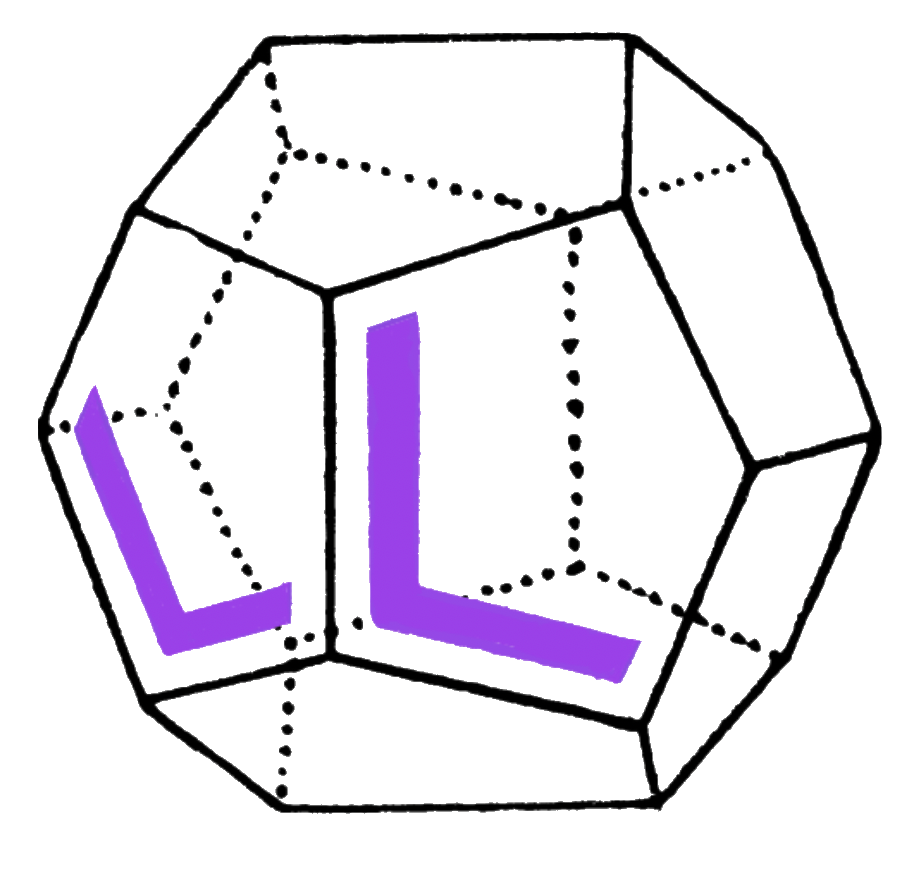
\includegraphics[width=2cm,height=2cm]{ll.png}}

    }}

\AddToShipoutPicture*
  {\put(470,737){

    \href{http://www.linearlibrary.net/CategoryTheory.pdf}{\texttt{.pdf file}}\\

  }}

\AddToShipoutPicture*
  {\put(470,752){
    \href{https://github.com/linlib/CategoryTheory/tree/main}{\texttt{.tex file}}\\

  }}

\AddToShipoutPicture*
  {\put(470,767){
    \href{http://www.linearlibrary.net/CategoryTheory.py}{\texttt{.py file}}

  }}

\AddToShipoutPicture*
  {\put(470,722){
    \href{https://github.com/linlib/CategoryTheory/tree/main}{\texttt{.lean project}}

  }}

\AddToShipoutPicture*
  {\put(470,737){

    \href{http://www.linearlibrary.net/CategoryTheory.pdf}{\texttt{.pdf file}}\\

  }}

\AddToShipoutPicture*
  {\put(415,752){
    \href{https://github.com/linlib/CategoryTheory/tree/main}{\texttt{.java file}}\\

  }}

\AddToShipoutPicture*
  {\put(415,767){
    \href{http://www.linearlibrary.net/CategoryTheory.py}{\texttt{.js file}}

  }}

\AddToShipoutPicture*
  {\put(415,737){
    \href{https://github.com/linlib/CategoryTheory/tree/main}{\texttt{.cpp file}}

  }}

\AddToShipoutPicture*
  {\put(415,722){
    \href{https://github.com/linlib/CategoryTheory/tree/main}{\texttt{.c file}}

  }}

\pagecolor{white}

\ \\
\ \\


\thispagestyle{empty} 

\AddToShipoutPicture*
    {\put(540,720){

    \href{http://www.linearlibrary.net}{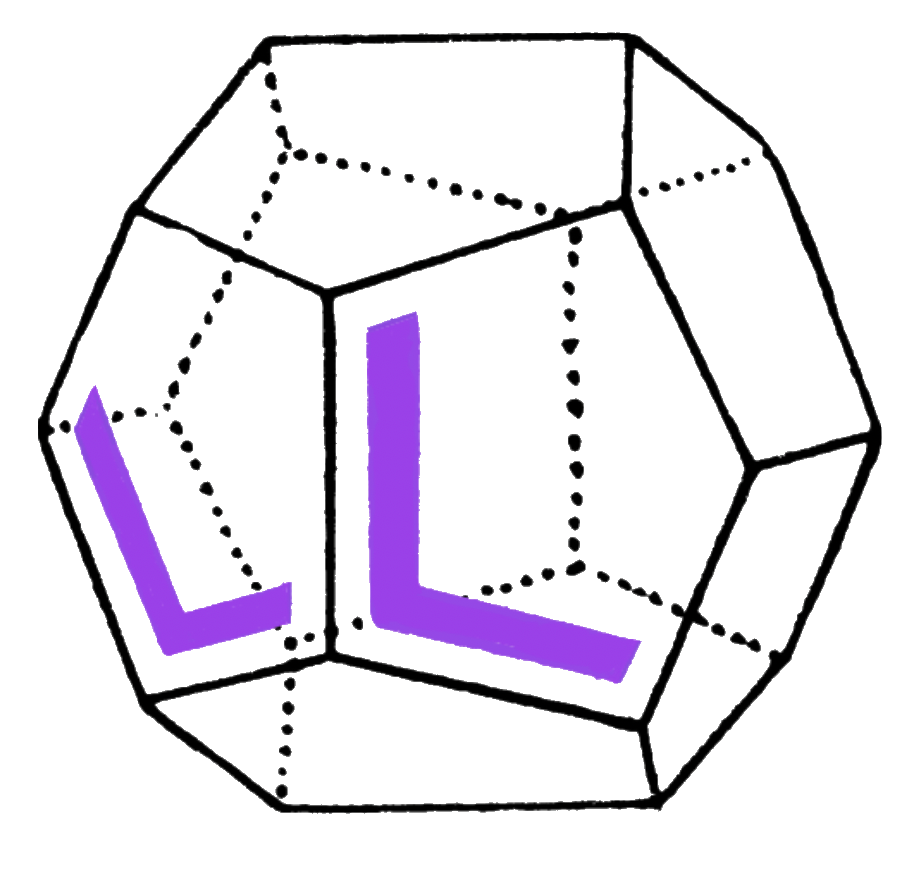
\includegraphics[width=2cm,height=2cm]{ll.png}}

    }}

\AddToShipoutPicture*
  {\put(470,767){
    \href{https://github.com/linlib/ThreeWhiteheadTheorems/StringDiagramGenerator.py}{\texttt{.py file}}
  }}

\AddToShipoutPicture*
  {\put(470,752){
    \href{https://github.com/linlib/ThreeWhiteheadTheorems/ThreeWhiteheadTheorems.tex}{\texttt{.tex file}}\\

  }}


\AddToShipoutPicture*
  {\put(470,737){

    \href{http://linearlibrary.net/ThreeWhiteheadTheorems/October19th.pdf}{\texttt{.pdf file}}\\

  }}

  \AddToShipoutPicture*
  {\put(470,722){
    \href{https://github.com/linlib/ThreeWhiteheadTheorems/ThreeWhiteheadTheorems.lean}{\texttt{.lean file}}

  }}

\ \\

%LEAN: 
\begin{center}
\begin{tcolorbox}[width=5.8in,colback={white},coltitle=white]
\begin{center}
\ \\
\scalebox{3}{\texttt{𝔾𝕖𝕠𝕞𝕖𝕥𝕣𝕚𝕔 𝕄𝕒𝕡𝕤 𝕚𝕟 ℍ𝕚𝕘𝕙𝕖𝕣 𝕋𝕠𝕡𝕠𝕤 𝕋𝕙𝕖𝕠𝕣𝕪}}\\
\ \\
\end{center}
\end{tcolorbox}
\end{center}
\ \\

\begin{center}
  \begin{tabular}{ c c }
  \multicolumn{2}{c}{$\texttt{Topological \ Duality}$}\\
  \hline
  $\texttt{open\ map}$ & $\texttt{closed\ map}$  \\ 
  $\texttt{universally\ open\ map}$ & $\texttt{universally\ closed\ map}$\\
  $\texttt{unramified\ map}$ & $\texttt{separated\ map}$ \\  
  $\texttt{étale\ map}$ & $\texttt{proper\ map}$  \\
  \hline
  \end{tabular}
  \end{center}

%LEAN: 
\begin{center}
\begin{tcolorbox}[width=4.13in,colback={white},coltitle=white]
\scalebox{2}{𝔼𛲔 𝔻𝕖𝕒𝕟 𝕐𝕠𝕦𝕟𝕘}
\end{tcolorbox}
\end{center}



\thispagestyle{empty}


\newpage
\section{Introduction}


\newpage
\section{Unicode}

Here is a list of the unicode characters I will use:

{\footnotesize
\begin{center}
\begin{tabular}{|| l || l || l || l ||} 
\hline
$\texttt{Symbol}$ & $\texttt{Unicode}$ & \texttt{VSCode shortcut} & $\texttt{Use}$\\
\hline
\hline
\multicolumn{4}{||c||}{\texttt{Lean's Kernel}} \\
\hline
\hline
× & 2A2F & \backslash\texttt{times} & Product of types\\
\hline
→ & 2192 & \backslash\texttt{rightarrow}  & Hom of types\\
\hline
⟨,⟩ & 27E8,27E9 & \backslash\texttt{langle},\backslash\texttt{rangle}  & Product term introduction\\
\hline
↦ & 21A6 &\backslash\texttt{mapsto}  & Hom term introduction\\
\hline
∧ & 2227 &\backslash\texttt{wedge}  & Conjunction \\
\hline
∨ & 2228 &\backslash\texttt{vee}  & Disjunction \\
\hline
∀ & 2200 &\backslash\texttt{forall}  & Universal quantification \\
\hline
∃ & 2203 &\backslash\texttt{exists}  & Existential quantification\\
\hline
¬ & 00AC &\backslash\texttt{neg}  & Negation\\
\hline
\hline
\multicolumn{4}{||c||}{\texttt{Variables and Constants}} \\
\hline
\hline
ᵃ,ᵇ,ᶜ,...,ᶻ & 1D52,1D56 &\iffalse\backslash{}^{$\wedge$}\texttt{a},{\backslash{}}^{$\wedge$}\texttt{b},\backslash{}^{$\wedge$}\texttt{c},...\backslash{}^{$\wedge$}\texttt{z}\fi  & Variables and constants \\
\hline
⁰,¹,²,³,⁴,⁵,⁶,⁷,⁸,⁹ & 1D52,1D56 & \iffalse\backslash\wedge\texttt{0},\backslash{}^{$\wedge$}\texttt{1},\backslash{}^{$\wedge$}\texttt{2},...,\backslash{}^{$\wedge$}\texttt{9}\fi  & Variables and constants \\
\hline
⁻ & 207B & \iffalse\backslash\wedge\texttt{-},\fi  & Variables and constants \\
\hline
₀,₁,₂,₃,₄,₅,₆,₇,₈,₉ & 2080 - 2089 & \backslash\texttt{0}-\backslash\texttt{9} & Variables and constants\\
\hline
𝔸,...,ℤ & 1D538 & \backslash\texttt{bbA},...,\backslash\texttt{bbZ} &  Variables and constants \\
\hline
𝕒,...,𝕫 & 1D552 & \backslash\texttt{bba},...,\backslash\texttt{bbz} & Variables and constants \\
\hline
\iffalse 𝐀,...,𝐙 & 1D41A & \backslash\texttt{bfA},...,\backslash\texttt{bfZ} & Variables and constants \\
\hline
𝐚,...,𝐳 & 1D41A & \backslash\texttt{bfa},...,\backslash\texttt{bfz} & Variables and constants \\
\hline \fi
\texttt{α}-\texttt{ω},\texttt{A}-\texttt{Ω} & 03B1-03C9 & & Variables and constants\\
\hline
\hline
\multicolumn{4}{||c||}{\texttt{Categories and Bicategories}} \\
\hline
\hline
 𝟙 & 1D7D9 & \backslash\texttt{b1}  & The identity morphism\\
\hline
 ≫ & 2218 & & Composition\\
\hline
   &  &  & Composition\\
\hline
   &  &  & Composition\\
\hline
 \multicolumn{4}{||c||}{\texttt{Adjunctions}} \\
\hline
\hline\iffalse
⇄ & 21C4 & \backslash\texttt{rightleftarrows}  & Adjunctions \\
\hline
⇆ & 21C6 & \backslash\texttt{leftrightarrows}  & Adjunctions \\
\hline\fi
𛲔 & 1BC94 &  & Right adjoints\\
\hline
ॱ & 0971 &  & Left adjoints \\
\hline
⊣ & 22A3 & \backslash\texttt{dashv}  & The condition that two functors are adjoint \\
\hline
\hline
\multicolumn{4}{||c||}{\texttt{Monads and Comonads}} \\
\hline
\hline
?,¿ & 003F, 00BF & ?,\backslash\texttt{?}  & The corresponding (co)monad of an adjunction\\
\hline
!,¡ & 0021, 00A1 & !, \backslash\texttt{!}  & The (co)-Eilenberg-(co)-Moore adjunction \\
\hline
ꜝ,ꜞ & A71D, A71E &  & The (co)AdjMon maps\\
\hline
\hline
\multicolumn{4}{||c||}{\texttt{Miscellaneous}} \\
\hline
\hline
\iffalse ∼ & 223C & \backslash\texttt{sim} & Homotopies \\
\hline\fi
≃ & 2243 & \backslash\texttt{equiv}  & Equivalences \\
\hline
≅ & 2245 & \backslash\texttt{cong}   & Isomorphisms \\
\hline
⊥ & 22A5 & \backslash\texttt{bot}    & The overobject classifier \\
\hline
∞ & 221E & \backslash\texttt{infty}  & Infinity categories and infinity groupoids\\ 
 \hline
\end{tabular}
\end{center}}

Of these, the characters $\texttt{ꜝ,ꜞ,𛲔}$ and $\texttt{ॱ}$ do not have VSCode shortcuts, and so I provide alternatives for them. Possibly they will have to be changed if this work assimilates into a larger project.\\

It is not possible to copy the from the pdf to the clipboard while preserving the integrity of the code. To see the official Lean 4 file please click the link on the top right of the front page or \href{https://github.com/linlib/CategoryTheory/tree/main}{this}.



%LEAN: 
\begin{center}
\begin{tcolorbox}[width=5in,colback={white},title={\begin{center}\texttt{Lean \thelcounter} \addtocounter{lcounter}{1}  \end{center}},colbacktitle=Blue,coltitle=black]
\begin{minted}[breaklines, escapeinside=||]{lean}


import Mathlib.CategoryTheory.Bicategory.Basic
import Mathlib.CategoryTheory.Types 
import Mathlib.CategoryTheory.DiscreteCategory
import Mathlib.Combinatorics.Quiver.Basic
import Mathlib.CategoryTheory.Category.Init
import Aesop
import Init
import Mathlib.CategoryTheory.DiscreteCategory
import Mathlib.CategoryTheory.Bicategory.Strict
import Mathlib.CategoryTheory.ConcreteCategory.Bundled
import Mathlib.CategoryTheory.Functor.Basic
import Init.Core
import Mathlib.CategoryTheory.Category.Cat

import TheWhiteheadTheorem

-- #check 
-- #

\end{minted}
\end{tcolorbox}
\end{center}


\newpage
\begin{center}

\pagecolor{white}
\color{black}




\end{center}

\thispagestyle{empty}




\newpage
\pagecolor{white}
\color{black}
\ \\
\ \\
\thispagestyle{empty}
\begin{center}
Copyright\ \textcopyright \ June 2023 Elliot Dean Young.\ All rights reserved.\\
\end{center}
\large %%%%%%%% HERE IS THE large LARGE size textsize set text size
\newpage 
\ \\
\ \\
\ \\
\ \\
\ \\
\ \\
\ \\
\ \\
\ \\
\ \\
\ \\
\thispagestyle{empty}
 



















\newpage










\thispagestyle{empty} 

\AddToShipoutPicture*
    {\put(540,720){

    \href{http://www.linearlibrary.net}{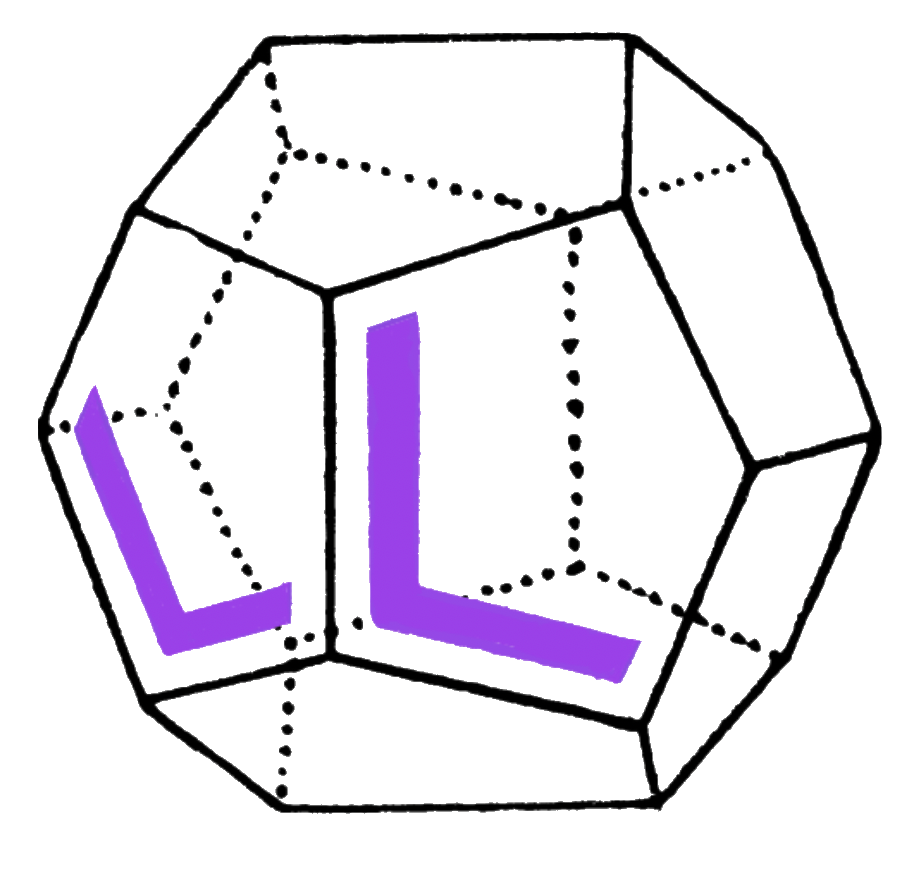
\includegraphics[width=2cm,height=2cm]{ll.png}}

    }}

\AddToShipoutPicture*
  {\put(470,737){

    \href{http://www.linearlibrary.net/CategoryTheory.pdf}{\texttt{.pdf file}}\\

  }}

\AddToShipoutPicture*
  {\put(470,752){
    \href{https://github.com/linlib/CategoryTheory/tree/main}{\texttt{.tex file}}\\

  }}

\AddToShipoutPicture*
  {\put(470,767){
    \href{http://www.linearlibrary.net/CategoryTheory.py}{\texttt{.py file}}

  }}

\AddToShipoutPicture*
  {\put(470,722){
    \href{https://github.com/linlib/CategoryTheory/tree/main}{\texttt{.lean project}}

  }}

\AddToShipoutPicture*
  {\put(470,737){

    \href{http://www.linearlibrary.net/CategoryTheory.pdf}{\texttt{.pdf file}}\\

  }}

\AddToShipoutPicture*
  {\put(415,752){
    \href{https://github.com/linlib/CategoryTheory/tree/main}{\texttt{.java file}}\\

  }}

\AddToShipoutPicture*
  {\put(415,767){
    \href{http://www.linearlibrary.net/CategoryTheory.py}{\texttt{.js file}}

  }}

\AddToShipoutPicture*
  {\put(415,737){
    \href{https://github.com/linlib/CategoryTheory/tree/main}{\texttt{.cpp file}}

  }}

\AddToShipoutPicture*
  {\put(415,722){
    \href{https://github.com/linlib/CategoryTheory/tree/main}{\texttt{.c file}}

  }}

\pagecolor{white}

\ \\
\ \\


\thispagestyle{empty} 

\AddToShipoutPicture*
    {\put(540,720){

    \href{http://www.linearlibrary.net}{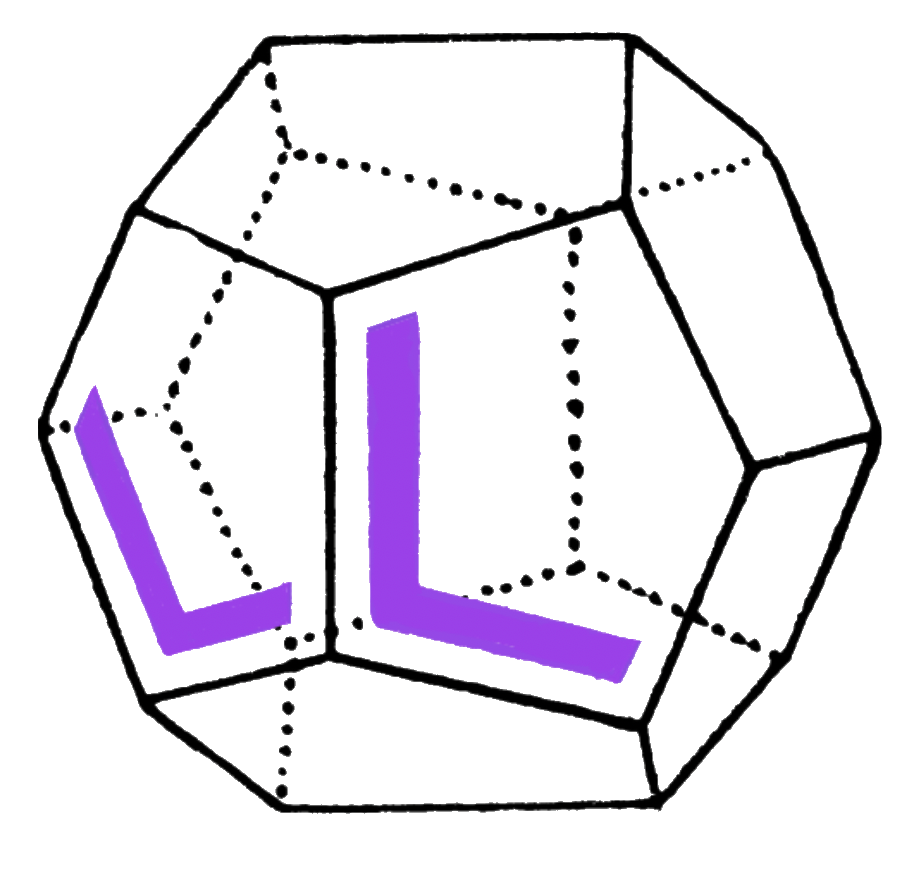
\includegraphics[width=2cm,height=2cm]{ll.png}}

    }}

\AddToShipoutPicture*
  {\put(470,767){
    \href{https://github.com/linlib/ThreeWhiteheadTheorems/StringDiagramGenerator.py}{\texttt{.py file}}
  }}

\AddToShipoutPicture*
  {\put(470,752){
    \href{https://github.com/linlib/ThreeWhiteheadTheorems/ThreeWhiteheadTheorems.tex}{\texttt{.tex file}}\\

  }}


\AddToShipoutPicture*
  {\put(470,737){

    \href{http://linearlibrary.net/ThreeWhiteheadTheorems/October19th.pdf}{\texttt{.pdf file}}\\

  }}

  \AddToShipoutPicture*
  {\put(470,722){
    \href{https://github.com/linlib/ThreeWhiteheadTheorems/ThreeWhiteheadTheorems.lean}{\texttt{.lean file}}

  }}

\ \\

%LEAN: 
\begin{center}
\begin{tcolorbox}[width=5.8in,colback={white},coltitle=white]
\begin{center}
\ \\
\scalebox{1.5}{\texttt{𝔾𝕖𝕠𝕞𝕖𝕥𝕣𝕚𝕔 𝕄𝕒𝕡𝕤 𝕚𝕟 𝕊𝕥𝕒𝕓𝕝𝕖 ℍ𝕠𝕞𝕠𝕥𝕠𝕡𝕪 𝕋𝕙𝕖𝕠𝕣𝕪}}\\
\ \\
\end{center}
\end{tcolorbox}
\end{center}
\ \\


%LEAN: 
\begin{center}
\begin{tcolorbox}[width=4.13in,colback={white},coltitle=white]
\scalebox{2}{𝔼𛲔 𝔻𝕖𝕒𝕟 𝕐𝕠𝕦𝕟𝕘}
\end{tcolorbox}
\end{center}


\begin{center}
\texttt{Plans to establish some basic features}\\
\texttt{of geometric maps between stable homotopy}\\
\texttt{categories after the construction of}\\
\texttt{six variations of the stable (∞,1)-category}\\
\texttt{of spectra as a term of type ∞-Cat.α,}\\
\texttt{with extensive use of Mathlib's pro-finite}\\
\texttt{and ind-finite constructions, monoidal}\\
\texttt{categories, adjunctions, monads, comonads,}\\
\texttt{Eilenberg-Moore theory, simplicial sets,}\\
\texttt{and }
\end{center}


\thispagestyle{empty}


\newpage
\section{Introduction}

In the first of four outlines concerning the development of the $\texttt{linearlibrary}$ project, whose main goal was {\bf prove the Whitehead theorem and exactness of the Puppe sequence for for Lean 4's homotopy category of based connected simplicial sets with the Kan lifting condition}, we established six variations of a common theorem:

\begin{enumerate}
\item $\texttt{D(}$∞$\texttt{-Cat) : Cat}$ is deloopable internal categories in itself.
\item $\texttt{D(}$∞$\texttt{-Cat/C) : Cat}$ is deloopable internal $\texttt{C}$-presheaves in itself. 
\item $\texttt{D(}$∞$\texttt{-Grpd) : Cat}$ is deloopable internal groupoids in itself.
\item $\texttt{D(}$∞$\texttt{-Grpd/G) : Cat}$ is deloopable internal $\texttt{G}$-presheaves in itself.
\item $\texttt{D(}$∞$\texttt{-Grpd₀) : Cat}$ is deloopable internal groupoids in itself.
\item $\texttt{D(}$∞$\texttt{-Grpd₀/G) : Cat}$ is deloopable internal $\texttt{G}$-presheaves in itself.
\end{enumerate}

In the second document, we outlined the construction of six further categories:

\begin{enumerate}
\item  
\item 
\item 
\item 
\end{enumerate}

In this document, we examine geometric maps between stable homotopy categories (particular (∞,1)-categories). A good reference for the work here is Lurie's ``Higher Algebra''. 

\begin{enumerate}
\item https://www.math.ias.edu/~lurie/papers/HA.pdf
\item 
\end{enumerate}

The main conditions on geometric map that we study are listed in the table below:


{\footnotesize
\begin{center}
\begin{tabular}{|| l || l || l || l ||} 
\hline
$\texttt{Symbol}$ & $\texttt{Unicode}$ & \texttt{VSCode shortcut} & $\texttt{Use}$\\
\hline
\hline
\multicolumn{4}{||c||}{\texttt{Lean's Kernel}} \\
\hline
\hline

 \hline
\end{tabular}
\end{center}}

\newpage
\section{Unicode}

Here is a list of the unicode characters I will use:

{\footnotesize
\begin{center}
\begin{tabular}{|| l || l || l || l ||} 
\hline
$\texttt{Symbol}$ & $\texttt{Unicode}$ & \texttt{VSCode shortcut} & $\texttt{Use}$\\
\hline
\hline
\multicolumn{4}{||c||}{\texttt{Lean's Kernel}} \\
\hline
\hline
× & 2A2F & \backslash\texttt{times} & Product of types\\
\hline
→ & 2192 & \backslash\texttt{rightarrow}  & Hom of types\\
\hline
⟨,⟩ & 27E8,27E9 & \backslash\texttt{langle},\backslash\texttt{rangle}  & Product term introduction\\
\hline
↦ & 21A6 &\backslash\texttt{mapsto}  & Hom term introduction\\
\hline
∧ & 2227 &\backslash\texttt{wedge}  & Conjunction \\
\hline
∨ & 2228 &\backslash\texttt{vee}  & Disjunction \\
\hline
∀ & 2200 &\backslash\texttt{forall}  & Universal quantification \\
\hline
∃ & 2203 &\backslash\texttt{exists}  & Existential quantification\\
\hline
¬ & 00AC &\backslash\texttt{neg}  & Negation\\
\hline
\hline
\multicolumn{4}{||c||}{\texttt{Variables and Constants}} \\
\hline
\hline
ᵃ,ᵇ,ᶜ,...,ᶻ & 1D52,1D56 &\iffalse\backslash{}^{$\wedge$}\texttt{a},{\backslash{}}^{$\wedge$}\texttt{b},\backslash{}^{$\wedge$}\texttt{c},...\backslash{}^{$\wedge$}\texttt{z}\fi  & Variables and constants \\
\hline
⁰,¹,²,³,⁴,⁵,⁶,⁷,⁸,⁹ & 1D52,1D56 & \iffalse\backslash\wedge\texttt{0},\backslash{}^{$\wedge$}\texttt{1},\backslash{}^{$\wedge$}\texttt{2},...,\backslash{}^{$\wedge$}\texttt{9}\fi  & Variables and constants \\
\hline
⁻ & 207B & \iffalse\backslash\wedge\texttt{-},\fi  & Variables and constants \\
\hline
₀,₁,₂,₃,₄,₅,₆,₇,₈,₉ & 2080 - 2089 & \backslash\texttt{0}-\backslash\texttt{9} & Variables and constants\\
\hline
𝔸,...,ℤ & 1D538 & \backslash\texttt{bbA},...,\backslash\texttt{bbZ} &  Variables and constants \\
\hline
𝕒,...,𝕫 & 1D552 & \backslash\texttt{bba},...,\backslash\texttt{bbz} & Variables and constants \\
\hline
\iffalse 𝐀,...,𝐙 & 1D41A & \backslash\texttt{bfA},...,\backslash\texttt{bfZ} & Variables and constants \\
\hline
𝐚,...,𝐳 & 1D41A & \backslash\texttt{bfa},...,\backslash\texttt{bfz} & Variables and constants \\
\hline \fi
\texttt{α}-\texttt{ω},\texttt{A}-\texttt{Ω} & 03B1-03C9 & & Variables and constants\\
\hline
\hline
\multicolumn{4}{||c||}{\texttt{Categories and Bicategories}} \\
\hline
\hline
 𝟙 & 1D7D9 & \backslash\texttt{b1}  & The identity morphism\\
\hline
 ≫ & 2218 & & Composition\\
\hline
   &  &  & Composition\\
\hline
   &  &  & Composition\\
\hline
 \multicolumn{4}{||c||}{\texttt{Adjunctions}} \\
\hline
\hline\iffalse
⇄ & 21C4 & \backslash\texttt{rightleftarrows}  & Adjunctions \\
\hline
⇆ & 21C6 & \backslash\texttt{leftrightarrows}  & Adjunctions \\
\hline\fi
𛲔 & 1BC94 &  & Right adjoints\\
\hline
ॱ & 0971 &  & Left adjoints \\
\hline
⊣ & 22A3 & \backslash\texttt{dashv}  & The condition that two functors are adjoint \\
\hline
\hline
\multicolumn{4}{||c||}{\texttt{Monads and Comonads}} \\
\hline
\hline
?,¿ & 003F, 00BF & ?,\backslash\texttt{?}  & The corresponding (co)monad of an adjunction\\
\hline
!,¡ & 0021, 00A1 & !, \backslash\texttt{!}  & The (co)-Eilenberg-(co)-Moore adjunction \\
\hline
ꜝ,ꜞ & A71D, A71E &  & The (co)AdjMon maps\\
\hline
\hline
\multicolumn{4}{||c||}{\texttt{Miscellaneous}} \\
\hline
\hline
\iffalse ∼ & 223C & \backslash\texttt{sim} & Homotopies \\
\hline\fi
≃ & 2243 & \backslash\texttt{equiv}  & Equivalences \\
\hline
≅ & 2245 & \backslash\texttt{cong}   & Isomorphisms \\
\hline
⊥ & 22A5 & \backslash\texttt{bot}    & The overobject classifier \\
\hline
∞ & 221E & \backslash\texttt{infty}  & Infinity categories and infinity groupoids\\ 
 \hline
\end{tabular}
\end{center}}

Of these, the characters $\texttt{ꜝ,ꜞ,𛲔}$ and $\texttt{ॱ}$ do not have VSCode shortcuts, and so I provide alternatives for them. Possibly they will have to be changed if this work assimilates into a larger project.\\

It is not possible to copy the from the pdf to the clipboard while preserving the integrity of the code. To see the official Lean 4 file please click the link on the top right of the front page or \href{https://github.com/linlib/CategoryTheory/tree/main}{this}.


%LEAN: 
\begin{center}
\begin{tcolorbox}[width=5in,colback={white},title={\begin{center}\texttt{Lean \thelcounter} \addtocounter{lcounter}{1}  \end{center}},colbacktitle=Blue,coltitle=black]
\begin{minted}[breaklines, escapeinside=||]{lean}

import Mathlib.CategoryTheory.Bicategory.Basic
import Mathlib.CategoryTheory.Types 
import Mathlib.CategoryTheory.DiscreteCategory
import Mathlib.Combinatorics.Quiver.Basic
import Mathlib.CategoryTheory.Category.Init
import Aesop
import Init
import Mathlib.CategoryTheory.DiscreteCategory
import Mathlib.CategoryTheory.Bicategory.Strict
import Mathlib.CategoryTheory.ConcreteCategory.Bundled
import Mathlib.CategoryTheory.Functor.Basic
import Init.Core
import Mathlib.CategoryTheory.Category.Cat

import TheWhiteheadTheorem

-- #check 
-- #

\end{minted}
\end{tcolorbox}
\end{center}


\newpage
\begin{center}

\pagecolor{white}
\color{black}




\end{center}

\thispagestyle{empty}




\newpage
\pagecolor{white}
\color{black}
\ \\
\ \\
\thispagestyle{empty}
\begin{center}
Copyright\ \textcopyright \ June 2023 Elliot Dean Young and Jiazhen Xia.\ All rights reserved.\\
\end{center}
\large %%%%%%%% HERE IS THE large LARGE size textsize set text size
\newpage 
\ \\
\ \\
\ \\
\ \\
\ \\
\ \\
\ \\
\ \\
\ \\
\ \\
\ \\
\thispagestyle{empty}
 




 


\newpage
\section{Unicode}

Lean 4 uses unicode, and this entails an extensive catalogue of characters to choose from. Here is a list of the unicode characters we will use:

{\footnotesize
\begin{center}
\begin{tabular}{|| l || l || l || l ||} 
\hline
$\texttt{Symbol}$ & $\texttt{Unicode}$ & \texttt{VSCode shortcut} & $\texttt{Use}$\\
\hline
\hline
\multicolumn{4}{||c||}{\texttt{Lean's Kernel}} \\
\hline
\hline
× & 2A2F & \backslash\texttt{times} & Product of types\\
\hline
→ & 2192 & \backslash\texttt{rightarrow}  & Hom of types\\
\hline
⟨,⟩ & 27E8,27E9 & \backslash\texttt{langle},\backslash\texttt{rangle}  & Product term introduction\\
\hline
↦ & 21A6 &\backslash\texttt{mapsto}  & Hom term introduction\\
\hline
∧ & 2227 &\backslash\texttt{wedge}  & Conjunction \\
\hline
∨ & 2228 &\backslash\texttt{vee}  & Disjunction \\
\hline
∀ & 2200 &\backslash\texttt{forall}  & Universal quantification \\
\hline
∃ & 2203 &\backslash\texttt{exists}  & Existential quantification\\
\hline
¬ & 00AC &\backslash\texttt{neg}  & Negation\\
\hline
\hline
\multicolumn{4}{||c||}{\texttt{Variables and Constants}} \\
\hline
\hline
ᵃ,ᵇ,ᶜ,...,ᶻ & 1D52,1D56 &\iffalse\backslash{}^{\wedge}\texttt{a},\backslash{}^{\wedge}\texttt{b},\backslash{}^{\wedge}\texttt{c},...\backslash{}^{\wedge}\texttt{z}\fi  & Variables and constants \\
\hline
⁰,¹,²,³,⁴,⁵,⁶,⁷,⁸,⁹ & 1D52,1D56 & \iffalse \backslash\wedge\texttt{0},\backslash{}^{\wedge}\texttt{1},\backslash{}^{\wedge}\texttt{2},...,\backslash{}^{\wedge}\texttt{9} \fi & Variables and constants \\
\hline
⁻ & 207B &\iffalse \backslash\wedge\texttt{-},\fi  & Variables and constants \\
\hline
₀,₁,₂,₃,₄,₅,₆,₇,₈,₉ & 2080 - 2089 & \backslash\texttt{0}-\backslash\texttt{9} & Variables and constants\\
\hline
𝔸,...,ℤ & 1D538 &  &  \\
\hline
𝕒,...,𝕫 & 1D552 &  &  \\
\hline
𝐀,...,𝐙 & 1D41A &  &  \\
\hline
𝐚,...,𝐳 & 1D41A &  &  \\
\hline
\texttt{α}-\texttt{ω},\texttt{A}-\texttt{Ω} & 03B1-03C9 & & Variables and constants\\
\hline
\hline
\multicolumn{4}{||c||}{\texttt{Categories}} \\
\hline
\hline
 𝟙 & 1D7D9 & \backslash\texttt{b1}  & The identity morphism\\
\hline
 ∘ & 2218 & \backslash\texttt{circ}  & Composition\\
 \hline
 \hline
 \multicolumn{4}{||c||}{\texttt{Twocategories}} \\
 \hline 
 \hline
 𝟏 & 1D7CF &   & Horizontal identity map \\ %are these even necessary?
 \hline
 • & 2022  & \backslash\texttt{smul}  & Horizontal composition of objects\\ %are these even necessary?
 \hline
 ∙ & 2219  &   & Horizontal composition of morphisms\\ %are these even necessary?
  \hline
  \hline
 \multicolumn{4}{||c||}{\texttt{Adjunctions}} \\
\hline
\hline
⇄ & 21C4 & \backslash\texttt{rightleftarrows}  & Adjunctions \\
\hline
⇆ & 21C6 & \backslash\texttt{leftrightarrows}  & Adjunctions \\
\hline
𛲔 & 1BC94 &  & Right adjoints\\
\hline
ॱ & 0971 &  & Left adjoints \\
\hline
⊣ & 22A3 & \backslash\texttt{dashv}  & The condition that two functors are adjoint \\
\hline
\hline
\multicolumn{4}{||c||}{\texttt{Monads and Comonads}} \\
\hline
\hline
?,¿ & 003F, 00BF & ?,\backslash\texttt{?}  & The corresponding (co)monad of an adjunction\\
\hline
!,¡ & 0021, 00A1 & !, \backslash\texttt{!}  & The (co)-Eilenberg-(co)-Moore adjunction \\
\hline
ꜝ,ꜞ & A71D, A71E &  & The (co)exponential maps\\
\hline
\hline
\multicolumn{4}{||c||}{\texttt{Miscellaneous}} \\
\hline
\hline
∼ & 223C & \backslash\texttt{sim} & Homotopies \\
\hline
≃ & 2243 & \backslash\texttt{equiv}  & Equivalences \\
\hline
≅ & 2245 & \backslash\texttt{cong}  & Isomorphisms \\
\hline
⊥ & 22A5 & \backslash\texttt{bot}  & The overobject classifier \\
\hline
∞ & 221E & \backslash\texttt{infty}  & Infinity categories and infinity groupoids\\ 
 \hline
\end{tabular}
\end{center}}

\iffalse
https://en.wikipedia.org/wiki/D-module
\fi

Of these, the characters $\texttt{ꜝ,ꜞ,𛲔,ॱ,𝟏}$, and $\texttt{∙}$ do not have VSCode shortcuts, and so we provide alternatives for them.\\

It is not possible to copy the from the pdf to the clipboard while preserving the integrity of the code. To see the official Lean 4 file please click the link on the top right of the front page or \href{https://github.com/linlib/CategoryTheory/tree/main}{this}.

\ \\
\ \\
\ \\


\part{PROPER AND ÉTALE MAPS FOR ∞-CATEGORIES}

Next we introduce the concept of a locus, which is much like a pullback system or topos, but which is both complete and cocomplete and features two adjunctions in its maps. ... 

\begin{enumerate}
\item $\texttt{[-,}$∞$\texttt{\_(}$∞$\texttt{-Cat)] : D(}$∞$\texttt{-Cat) ⭢ D(}$∞$\texttt{-Cat)}$ always has two adjunctions so that ∞-categories produce a locus.
\item The locus obtained from monoids in the homotopy category of spectra is to do with equations and unknowns
\item The locus obtained from comonoids in the homotopy category of spectra is better suited to be a 
\item The locus of analytic spaces, in which proper is equivalent to étale and to a condition involving trace
\end{enumerate} We will mainly be interested in two different loci: the locus of ∞-categories, the locus of comonoid objects in the homotopy category of spectra, the (opposite) locus of monoid objects in the homotopy category of spectra. Each of these obeys the fundamental theorems about loci 

I would like to make special thanks in this section to Paul Taylor and Martin Escardo, whose studies of adjoint-based conditions related to compactness and etaleness in locales contain many gems of point-set topology. Taylor's paper on these matters can be found \href{https://paultaylor.eu/ASD/foufct/foufct.pdf}{here} and Escardo's central paper on these matters can be found \href{https://www.cs.bham.ac.uk/~mhe/papers/barbados.pdf}{here}. Here we have expressed compactness as the existence of a topological adjoint and etaleness (compare with Paul Taylor's $\textit{overt}$) as the existence of an adjoint continuous in the scott topology. 



\chapter{The Free Locus}



\chapter{Filtered Colimits and Cofiltered Limits}

\iffalse
\begin{enumerate}
\item It may be possible to show that the free pullback system on a cartesian closed pullback system is cartesian closed.
\item Finite limits and filtered colimits commute in a pullback\_system.
\item Freely adding in new pullbacks (finite limits) to category is an important construction.
\item Filtered colimits are those colimits that commute with finite limits.
\item The free pullback system map of a functor has a right adjoint, and yet it may not produce a commutative diagram featuring the original functor. 
\item The condition expressing that it does is that the original functor preserve filtered colimits. We say a functor is continuous if it preserves filtered colimits.
\item If a left adjoint map of loci has a right adjoint that preserves filtered colimits, then it should be called a continuous adjunction.
\item 
\end{enumerate}
\fi

%LEAN: 
\begin{center}
\begin{tcolorbox}[width=5in,colback={white},title={\begin{center}\texttt{Lean \thelcounter} \addtocounter{lcounter}{1}  \end{center}},colbacktitle=Blue,coltitle=black]
\begin{minted}[breaklines, escapeinside=||]{lean}

def completion : adjunction ℂ𝕒𝕥 := sorry

\end{minted}
\end{tcolorbox}
\end{center}

%LEAN: 
\begin{center}
\begin{tcolorbox}[width=5in,colback={white},title={\begin{center}\texttt{Lean \thelcounter} \addtocounter{lcounter}{1}  \end{center}},colbacktitle=Blue,coltitle=black]
\begin{minted}[breaklines, escapeinside=||]{lean}

notation C "̂" => completion.Fst.Obj C
notation : 10000 "⟨" L "⟩" => completion.Snd.Obj L

\end{minted}
\end{tcolorbox}
\end{center}

\begin{theorem}
Let \texttt{Γ₁} and \texttt{Γ₂} be loci, and let \texttt{f : (ℂ𝕒𝕥.Hom (completion.Snd.Obj Γ₁) (completion.Snd.Obj Γ₂)).Obj}. The following are equivalent:
\begin{enumerate}
\item There is a commutative square featuring $\texttt{completion.ε Γ₁}$, $\texttt{completion.ε Γ₂}$, $\texttt{f}$ $\texttt{f̂}$.
\item $f$ preserves filtered colimits.
\end{enumerate}
\end{theorem}

\chapter{Continuous Maps}

\begin{enumerate}
\item When the free pullback system on a representation has an adjunction, we say that the original map is continuous. This is equivalent to preserving filtered colimits.
\item When a left adjoint has a continuous right adjoint, we say it is continuous
\end{enumerate}

\chapter{Open Maps and Closed Maps}

\begin{enumerate}
\item An analysis of open and closed maps of locales reveals frobenius reciprocity as an important condition.
\item The main theorem of this section says that frobenius reciprocity is equivalent to the preservation of a hom.
\item 
\end{enumerate}

\begin{definition}
Let $\texttt{C, D : pullback\_system}$. Let $\texttt{f : Pul.Hom C D}$. $\texttt{f}$ is said to be open if \iffalse$\texttt{∀\_(f)𛲔.Obj (- \times\_(Γ) f) ≅\_() (∀\_(f)𛲔.Obj (-) \times -}$. \fi
\end{definition}



This definition is related to the definition of an \href{https://ncatlab.org/nlab/show/open+morphism}{open morphism of locales}.

\begin{definition}
Let $\texttt{C, D : Cat\_(D(Γ)).Obj}$. Let $\texttt{f : Cat\_(D(Γ)).Hom C D}$. $\texttt{f}$ is said to be closed if \iffalse$\texttt{∀\_(f)𛲔.Obj (- \times\_(Γ) f) ≅\_() (∀\_(f)𛲔.Obj (-) \times -}$\fi.
\end{definition}

This definition is related to the definition of a \href{https://ncatlab.org/nlab/show/closed+morphism}{closed morphism of locales}

\begin{theorem}[Open and closed maps]
Let $\texttt{C, D : Cat\_(D(Γ)).Obj}$. Let $\texttt{f : Cat\_(D(Γ)).Hom C D}$.
\begin{enumerate}
\item The following are equivalent: 
\begin{enumerate}
\item ??? \iffalse$\texttt{∀\_(f)𛲔.Obj (- \times\_(Γ) g) ≅\_(Cat.Hom) (∀\_(f)𛲔.Obj (-) \times\_(Γ) g)}$.\fi
\item ???
\end{enumerate}
\item The following are equivalent:
\begin{enumerate}
\item ??? \iffalse$\texttt{∃_(f)ॱ.Obj (- \times\_(Γ) f) ≅\_() (∃\_(f)ॱ.Obj X) \times Y}$.\fi
\item ???
\end{enumerate}
\end{enumerate}
\end{theorem}

\begin{proof}
\iffalse
  C(X, f([Y, Z]))
= D(exists_f X, [Y, Z])
= D(exists_f X prod Y, Z)
= D(Y prod exists_f X, Z)
= D(Y, [exists_f X, Z])
in a way which is natural in Z, and opnatural in X and Y.
\fi

and

\iffalse
  C(X, [fY, fZ])
= C(X prod fY, fZ)
= C(fY prod X, fZ)
= C(exists_f (fY prod X), Z)
in a way which is natural in Z, and opnatural in X and Y.
\fi
\end{proof}

\begin{theorem}
Let $\texttt{f : Loc.Hom X Y}$ and $\texttt{g : Loc.Hom Y Z}$ be maps of loci $\texttt{X : Loc.Obj}$ and $\texttt{Y : Loc.Obj}$. Then
\begin{enumerate}
\item If $\texttt{f}$ and $\texttt{g}$ are closed, then $\texttt{g ∘(Loc) f}$ is closed.
\item If $\texttt{f}$ and $\texttt{g}$ are open, then $\texttt{g ∘(Loc) f}$ is open.
\end{enumerate} 
\end{theorem}


To do:
\begin{enumerate}
\item Add in a classifier for closed maps.
\item Add in a classifier for open maps.
\end{enumerate}

\iffalse % "open if and only if postcomposition with an open is an open" "closed if and only if postcomposition with a closed is a closed"
\begin{theorem}
Let $\texttt{B}$ be a space and let $\texttt{f : X \rightarrow Y}$ be a map of $\texttt{S}$-spaces $\texttt{X}$ and $\texttt{Y}$. Then 
\begin{enumerate}
\item The following are equivalent:
\begin{enumerate}
\item $\texttt{F : 𝕃𝕠𝕔.Hom ()}$ is closed.
\item $\texttt{f • g}$ is closed when $\texttt{g}$ is closed.%%%how to define image?
\end{enumerate}
\item The following are equivalent:
\begin{enumerate}
\item $f$ is open.
\item $f • g$ is closed when $\texttt{g}$ is closed.%%%how to define image?
\end{enumerate}
\end{enumerate}
%%%phrase this for S-complete and R-cocomplete, and then have the space and algebra versions as corollares.
\end{theorem}

\begin{proof}

\end{proof}


\fi

\chapter{Universally Open and Universally Closed Maps}


\begin{enumerate}
\item Defining universally open and universally closed maps- we make use of the pullback in 𝕃𝕠𝕔.
\item The main theorem of this section says that:
\begin{enumerate}
\item A map $\texttt{f : Loc.Hom}$ is universally closed if and only if it has a right adjoint that preserves filtered colimits.
\item A map $\texttt{f : Loc.Hom}$ is universally open if and only if it has a left adjoint that preserves cofiltered limits.
\end{enumerate} 
\item We can also construct the properfication (topological completion; free addition of a ??? adjoint in the topological category)
\item Similarly we can construct the etalification (topological cocompletion; free addition of a ??? adjoint in the topological category)
\item We can take intersections via universally closed objects. (Tychonoff's theorem)
\item We can take unions via universally open objects. (Tychonoff's theorem)
\end{enumerate}


%LEAN: definition of universally closed
\begin{center}
\begin{tcolorbox}[width=5in,colback={white},title={\begin{center}\texttt{Lean \thelcounter} \addtocounter{lcounter}{1}  \end{center}},colbacktitle=Blue,coltitle=black]
\begin{minted}[breaklines, escapeinside=||]{lean}

\end{minted}
\end{tcolorbox}
\end{center}

%LEAN: definition of universally open
\begin{center}
\begin{tcolorbox}[width=5in,colback={white},title={\begin{center}\texttt{Lean \thelcounter} \addtocounter{lcounter}{1}  \end{center}},colbacktitle=Blue,coltitle=black]
\begin{minted}[breaklines, escapeinside=||]{lean}

\end{minted}
\end{tcolorbox}
\end{center}


\begin{theorem}
Let $\texttt{f : Loc.Hom X Y}$ and $\texttt{g : Loc.Hom X Z}$ be maps of loci.
\begin{enumerate}
\item If $\texttt{f}$ and $\texttt{g}$ are universally closed, then $\texttt{g ∘\_(Loc) f}$ is universally closed.
\item If $\texttt{f}$ and $\texttt{g}$ are universally open, then $\texttt{g ∘\_(Loc) f}$ is universall open. 
\end{enumerate}
\end{theorem}

This definition will be developed into a definition of universal and existential closure:

\begin{definition}
Let $\texttt{S}$ be a space and let $\texttt{X}$ be an $\texttt{S}$-space. 
\begin{enumerate}
\item universal closure produces a universally closed space in much the same way as $\texttt{[Cᵒᵖ,Set]}$.
\item existential closure produces a universally open space in much the same way as $\texttt{[Cᵒᵖ,Set]}$.
\end{enumerate}
\end{definition}

\begin{definition}
- intersection indexed by a universally closed object, the case for "over a point"
- union indexed by a universally open object, the case for "over a point"
\end{definition}

Tychonoff's theorem should produce intsersections by closed maps and unions by open maps. Here is where that will go:

\begin{theorem}[Tychnoff's Theorem (A)]
The following are equivalent:
\begin{enumerate}
\item $\texttt{X}$ is proper.
\item The projection $\texttt{X × Y → Y}$ is closed for each $\texttt{Y}$.
\item The projection $\texttt{X × [X,U] → [X,U]}$ is closed. 
\end{enumerate}
\end{theorem}

\begin{proof}

(1 => 2) The proper condition is closed under pullbacks. Proper implies closed.\\

(2 => 3) Take $\texttt{Y = [Xᵒᵖ, U]}$.\\

(3 => 1)  \iffalse Lan or Ran? $\texttt{(??? K Pnt τ\_(K)).Hom }$\fi $\texttt{Ran K Pnt τ\_(K)}$ sends $\texttt{K × [K, U]}$ to $\texttt{∀ : [K, U] → U}$. In particular it is continuous.\\

\end{proof}

\iffalse
- the hom of a universally closed space with ... is universally closed
- the product of an existentially closed space with ... is existentially closed.
\fi

\begin{theorem}[Tychnoff's Theorem (B)]
\iffalse
- the hom of a universally closed space with ... is universally closed
- the product of an existentially closed space with ... is existentially closed.
%%%phrase this for complete and cocomplete, and then have the space and algebra versions as corollares.
%%%the corollary may be a bit difficult since it involves ascertaining when the 
TFAE:
X is compact
X otimes Y -> Y is closed for each Y
X otimes [X, U^op] -> [X, U^op] is closed

(1 => 2)...

(2 => 3) 

(3 => 1) forall : [K, U] -> U is the universal image of in : K x [K, U] -> U. In particular it is continuous.
\fi
\end{theorem}

Further reading:
\begin{enumerate}
\item \href{https://en.wikipedia.org/wiki/Tube_lemma}{The tube lemma} says that projections of topological spaces $\texttt{f : X × K → K}$ with $\texttt{K}$ compact are closed.
\end{enumerate}

\chapter{Separated and Unramified Maps}

\begin{enumerate}
\item A map is called separated if the corresponding diagonal map is closed
\item A map is called unramified if the corresponding diagonal map is open
\item Separated is equivalent to universally separated.
\item Unramified is equivalent to universally unramified. 
\end{enumerate}

The negation of unramified is ramified, and the negation of separated is unseparated.

\begin{definition}
A map $\texttt{f : Loc.Hom E B}$ is called separated if ....
\end{definition}

%LEAN: 
\begin{center}
\begin{tcolorbox}[width=5in,colback={white},title={\begin{center}\texttt{Lean \thelcounter} \addtocounter{lcounter}{1}  \end{center}},colbacktitle=Blue,coltitle=black]
\begin{minted}[breaklines, escapeinside=||]{lean}

\end{minted}
\end{tcolorbox}
\end{center}

\begin{definition}
A map $\texttt{f : Loc.Hom E B}$ is called unramified if ....
\end{definition}

%LEAN: 
\begin{center}
\begin{tcolorbox}[width=5in,colback={white},title={\begin{center}\texttt{Lean \thelcounter} \addtocounter{lcounter}{1}  \end{center}},colbacktitle=Blue,coltitle=black]
\begin{minted}[breaklines, escapeinside=||]{lean}

\end{minted}
\end{tcolorbox}
\end{center}

\iffalse
\begin{theorem}
%Let $\texttt{S, X}$, and $\texttt{Y}$ be spaces, and let $\texttt{f : X}$ $\rightarrow$ $\texttt{S}$ and $\texttt{g : T \rightarrow S}$ be space maps. Then
\begin{enumerate}
\item If $\texttt{f : X \rightarrow S}$ is separated then $\texttt{f \times_S T : X \times_S T \rightarrow T}$ is separated.
\item If $\texttt{f : X \rightarrow S}$ is unramified then $\texttt{f \times_S T : X \times_S T \rightarrow T}$ is unramified.
\end{enumerate}
%%%phrase this for S-complete and R-cocomplete, and then have the space and algebra versions as corollares.
\end{theorem}

\begin{theorem}
Let $\texttt{f : X \rightarrow Y}$ be a space map. Then
\begin{enumerate}
\item The following are equivalent:
\begin{enumerate}
\item $\texttt{Δ\_(f) : Loc.Hom X  X ×\_Y X}$ is closed.
\item $\texttt{Δ\_(f) : Loc.Hom X X ×\_Y X}$ is universally closed.
\end{enumerate}
\item The following are equivalent:
\begin{enumerate}
\item $\texttt{Δ\_f : X \rightarrow X ×\_Y X}$ is open.
\item $\texttt{Δ\_f : X \rightarrow X ×\_Y X}$ is universally open.
\end{enumerate}
\end{enumerate}
%%%phrase this for S-complete and R-cocomplete, and then have the space and algebra versions as corollares.
\end{theorem}

\begin{proof}

\end{proof}


\begin{theorem}
Let $\texttt{f : X \rightarrow Y}$ and $\texttt{g : Y \rightarrow Z}$ be space maps. Then
\begin{enumerate}
\item If $\texttt{f : Loc.Hom X Y}$ and $\texttt{g : Loc.Hom Y Z}$ are separated, then $\texttt{g \circ f : Loc.Hom X Z}$ is separated.
\item If $\texttt{f : Loc.Hom X Y}$ and $\texttt{g : Loc.Hom Y }$ are unramified, then $\texttt{g \circ f : Loc.Hom X Z}$ is unramified.
\end{enumerate}
\end{theorem}

\begin{proof}

\end{proof}


\begin{theorem}
Let $\texttt{S}$ be a space, and let $\texttt{f : X \rightarrow S}$ and $\texttt{g : Y \rightarrow S}$ be $\texttt{S}$-spaces. Then
\begin{enumerate}
\item If $\texttt{X}$ is universally closed and $\texttt{\Gamma_S(Y)}$ is unramified then $\texttt{[X, \Gamma_S(Y)]}$ is unramified.
\item If $\texttt{X}$ is universally open and $\texttt{\Gamma_S(Y)}$ is separated then $\texttt{[X, \Gamma_S(Y)]}$ is separated.
\end{enumerate}
%%%phrase this for S-complete and R-cocomplete, and then have the space and algebra versions as corollares.
\end{theorem}

\begin{proof}

\end{proof}

\fi

\chapter{Proper Maps and Covering Spaces}

\begin{enumerate}
\item proper iff it has a continuous right adjoint and the corresponding diagonal map has a continuous right adjoint
\item etale if it has a continuous left adjoint and the corresponding diagonal map has a continuous left adjoint
\item An étale map should be an ind-limit of identity maps in a corresponding category of actions
\item A proper map should be a pro-limit of identity maps in a corresponding category of actions
\end{enumerate}


\begin{definition}
Let $\texttt{f : Loc.Hom X Y}$ be a space map. Then
\begin{enumerate}
\item We say $\texttt{f: Loc.Hom X Y}$ is proper if it is universally closed and separated.
\item We say $\texttt{f : Loc.Hom X Y}$ is étale if it is universally open and unramfied.
\end{enumerate}
\end{definition}

\iffalse
\begin{theorem}
Let $\texttt{X, Y}$, and $\texttt{S}$ be spaces, and let $\texttt{f : X \rightarrow S, g : Y \rightarrow S}$, and $\texttt{h : X \rightarrow Y}$ be space maps. Then
\begin{enumerate}
\item If $\texttt{f : X \rightarrow S}$ is separated and $\texttt{g : Y \rightarrow S}$ is proper, then $\texttt{h : X \rightarrow Y}$ is proper.
\item If $\texttt{f : X \rightarrow S}$ is unramified and $\texttt{g : Y \rightarrow S}$ is étale, then $\texttt{h : X \rightarrow Y}$ is étale.
\end{enumerate}
%%%phrase this for S-complete and R-cocomplete, and then have the space and algebra versions as corollares.
\end{theorem}

\iffalse
\begin{proof}
Consider that $f = (x \times_S Y) \circ f \times_Y X \circ \Delta_x$. $x \times_S Y$ is universally open since $x$ is universally open. $\Delta_x$ is universally open by assumption. That $f \times_S Y$ is universally open follows from that $Y$ is unramified.
\end{proof}
\fi

\begin{theorem}
Let $\texttt{X}, \texttt{S}$, and $\texttt{T}$ be spaces. Let $\texttt{f : Loc.Hom X S}$ and $\texttt{g : Loc.Hom T S}$ be space maps. Then
\begin{enumerate}
\item If $\texttt{f : Loc.Hom X S}$ is closed and $\texttt{g : Loc.Hom T S}$ is étale, then $\texttt{f ×\_S T : X ×\_S T \spacemap T}$ is closed.
\item If $\texttt{f : Loc.Hom X S}$ is open and $\texttt{g : Loc.Hom T S}$ is proper, then $\texttt{f ×\_S T : X ×\_S T \spacemap T}$ is open.
\end{enumerate} 
\end{theorem}

\begin{proof}

\end{proof}

\begin{proposition}
An étale map X -> Y is a filtered colimit of Y's in the linear category
\end{proposition}

\begin{corollary}
the dirac delta
\end{corollary}

\begin{proposition}
A proper map X -> Y is a cofiltered limit of Y's in the linear category
\end{proposition}

\begin{corollary}
the codirac delta
\end{corollary}
\fi

%TABLE
We can summarize the duality of the defintions and theorems in this section in a table:\\

\begin{center}
\begin{tabular}{ c c }
\multicolumn{2}{c}{$\texttt{Topological \ Duality}$}\\
\hline
$\texttt{open\ map}$ & $\texttt{closed\ map}$  \\ 
$\texttt{universally\ open\ map}$ & $\texttt{universally\ closed\ map}$\\
$\texttt{unramified\ map}$ & $\texttt{separated\ map}$ \\  
$\texttt{étale\ map}$ & $\texttt{proper\ map}$  \\
\hline
\end{tabular}
\end{center}

Further reading:
\begin{enumerate}
\item \href{https://ncatlab.org/nlab/show/Frobenius+reciprocity}{Frobenius reciprocity}
\item \href{https://mathoverflow.net/questions/404706/how-duality-follows-from-a-six-functor-formalism}{A mathoverflow question on the six-functor formalism}
\item \href{https://en.wikipedia.org/wiki/Verdier_duality}{Verdier duality}
\item \href{https://en.wikipedia.org/wiki/Coherent_duality}{Coherent duality}
\item \href{https://www.ams.org/journals/jams/1996-9-01/S0894-0347-96-00174-9/S0894-0347-96-00174-9.pdf}{Grothendieck Duality via Bousfield's Techniques (Amnon Neeman)}
\item \href{https://arxiv.org/pdf/1501.01999.pdf}{A paper on the 6-functor formalism}
\end{enumerate} 




\part{PROPER AND OVERT MAPS FOR ∞-GROUPOIDS}


\begin{enumerate}
\item note that [X,∞] <- [X, ∞] *always* has two adjunctions. 
\item so ∃ and ∀ always exist. 
\end{enumerate}

Special thanks is made in this section to Paul Taylor and Martin Escardo, whose studies of adjoint-based conditions related to compactness and etaleness in locales contains many gems of point-set topology. Taylor's main paper on these matters can be found \href{https://paultaylor.eu/ASD/foufct/foufct.pdf}{here} and Escardo's central paper on these matters can be found \href{https://www.cs.bham.ac.uk/~mhe/papers/barbados.pdf}{here}. Here we have expressed compactness as the existence of a topological adjoint and etaleness (compare with Paul Taylor's $\textit{overt}$) as the existence of an adjoint continuous in the scott topology. 


\chapter{The Free Locus}

\begin{enumerate}
\item The free pullback system freely adds in new pullbacks.
\end{enumerate}

\chapter{Filtered Colimits and Cofiltered Limits}

\begin{enumerate}
\item It may be possible to show that the free pullbacksystem on a cartesian closed pullback system is cartesian closed.
\item Finite limits and filtered colimits commute in a pullback system.
\item Freely adding in new pullbacks (finite limits) to category is an important construction.
\item Filtered colimits are those colimits that commute with finite limits.
\item The free pullback system map of a functor has a right adjoint, and yet it may not produce a commutative diagram featuring the original functor. 
\item The condition expressing that it does is that the original functor preserve filtered colimits. We say a functor is continuous if it preserves filtered colimits.
\item If a left adjoint map of loci has a right adjoint that preserves filtered colimits, then it should be called a continuous adjunction.
\item 
\end{enumerate}

%LEAN: 
\begin{center}
\begin{tcolorbox}[width=5in,colback={white},title={\begin{center}\texttt{Lean \thelcounter} \addtocounter{lcounter}{1}  \end{center}},colbacktitle=Blue,coltitle=black]
\begin{minted}[breaklines, escapeinside=||]{lean}

def completion : adjunction ℂ𝕒𝕥 := sorry

\end{minted}
\end{tcolorbox}
\end{center}

%LEAN: 
\begin{center}
\begin{tcolorbox}[width=5in,colback={white},title={\begin{center}\texttt{Lean \thelcounter} \addtocounter{lcounter}{1}  \end{center}},colbacktitle=Blue,coltitle=black]
\begin{minted}[breaklines, escapeinside=||]{lean}

notation C "̂" => completion.Fst.Obj C
notation : 10000 "⟨" L "⟩" => completion.Snd.Obj L

\end{minted}
\end{tcolorbox}
\end{center}

\begin{theorem}
Let \texttt{Γ₁} and \texttt{Γ₂} be loci, and let \texttt{f : (ℂ𝕒𝕥.Hom (completion.Snd.Obj Γ₁) (completion.Snd.Obj Γ₂)).Obj}. The following are equivalent:
\begin{enumerate}
\item There is a commutative square featuring $\texttt{completion.ε Γ₁}$, $\texttt{completion.ε Γ₂}$, $\texttt{f}$ $\texttt{f̂}$.
\item $f$ preserves filtered colimits.
\end{enumerate}
\end{theorem}

\chapter{Continuous Maps}

\begin{enumerate}
\item When the free pullback system on a representation has an adjunction, we say that the original map is continuous. This is equivalent to preserving filtered colimits.
\item When a left adjoint has a continuous right adjoint, we say it is continuous
\end{enumerate}

\chapter{Open Maps and Closed Maps}

\begin{enumerate}
\item An analysis of open and closed maps of locales reveals frobenius reciprocity as an important condition.
\item The main theorem of this section says that frobenius reciprocity is equivalent to the preservation of a hom.
\item 
\end{enumerate}

\begin{definition}
Let $\texttt{C, D : pullback\_system}$. Let $\texttt{f : Pul.Hom C D}$. $\texttt{f}$ is said to be open if \iffalse$\texttt{∀\_(f)𛲔.Obj (- \times\_(Γ) f) ≅\_() (∀\_(f)𛲔.Obj (-) \times -}$\fi. 
\end{definition}



This definition is related to the definition of an \href{https://ncatlab.org/nlab/show/open+morphism}{open morphism of locales}.

\begin{definition}
Let $\texttt{C, D : Cat\_(D(Γ)).Obj}$. Let $\texttt{f : Cat\_(D(Γ)).Hom C D}$. $\texttt{f}$ is said to be closed if \iffalse$\texttt{∀\_(f)𛲔.Obj (- \times\_(Γ) f) ≅\_() (∀\_(f)𛲔.Obj (-) \times -}$\fi.
\end{definition}

This definition is related to the definition of a \href{https://ncatlab.org/nlab/show/closed+morphism}{closed morphism of locales}

\begin{theorem}[Open and closed maps]
Let $\texttt{C, D : Cat\_(D(Γ)).Obj}$. Let $\texttt{f : Cat\_(D(Γ)).Hom C D}$.
\begin{enumerate}
\item The following are equivalent: 
\begin{enumerate}
\item ??? \iffalse$\texttt{∀\_(f)𛲔.Obj (- \times\_(Γ) g) ≅\_(Cat.Hom) (∀\_(f)𛲔.Obj (-) \times\_(Γ) g)}$.\fi
\item ???
\end{enumerate}
\item The following are equivalent:
\begin{enumerate}
\item ??? \iffalse$\texttt{∃_(f)ॱ.Obj (- \times\_(Γ) f) ≅\_() (∃\_(f)ॱ.Obj X) \times Y}$.\fi
\item ???
\end{enumerate}
\end{enumerate}
\end{theorem}

\begin{proof}


%LEAN: 
\begin{center}
\begin{tcolorbox}[width=5in,colback={white},title={\begin{center}\texttt{Lean \thelcounter} \addtocounter{lcounter}{1}  \end{center}},colbacktitle=Blue,coltitle=black]
\begin{minted}[breaklines, escapeinside=||]{lean}




/-

  [   X,     f([Y, Z])  ]_(C)
≅_(???) [∃_(f) X, [Y, Z]]
=_(???) D(exists_f X prod Y, Z)
=_(???) D(Y prod exists_f X, Z)
= D(Y, [exists_f X, Z])
in a way which is natural in Z, and opnatural in X and Y.

-/

\end{minted}
\end{tcolorbox}
\end{center}

and

\iffalse
  C(X, [fY, fZ])
= C(X prod fY, fZ)
= C(fY prod X, fZ)
= C(exists_f (fY prod X), Z)
in a way which is natural in Z, and opnatural in X and Y.
\fi
\end{proof}

\begin{theorem}
Let $\texttt{f : Loc.Hom X Y}$ and $\texttt{g : Loc.Hom Y Z}$ be maps of loci $\texttt{X : Loc.Obj}$ and $\texttt{Y : Loc.Obj}$. Then
\begin{enumerate}
\item If $\texttt{f}$ and $\texttt{g}$ are closed, then $\texttt{g ∘\_(Loc) f}$ is closed.
\item If $\texttt{f}$ and $\texttt{g}$ are open, then $\texttt{g ∘\_(Loc) f}$ is open.
\end{enumerate} 
\end{theorem}


To do:
\begin{enumerate}
\item Add in a classifier for closed maps.
\item Add in a classifier for open maps.
\end{enumerate}

\iffalse % "open if and only if postcomposition with an open is an open" "closed if and only if postcomposition with a closed is a closed"
\begin{theorem}
Let $\texttt{B}$ be a space and let $\texttt{f : X \rightarrow Y}$ be a map of $\texttt{S}$-spaces $\texttt{X}$ and $\texttt{Y}$. Then 
\begin{enumerate}
\item The following are equivalent:
\begin{enumerate}
\item $\texttt{F : 𝕃𝕠𝕔.Hom ()}$ is closed.
\item $\texttt{f • g}$ is closed when $\texttt{g}$ is closed.%%%how to define image?
\end{enumerate}
\item The following are equivalent:
\begin{enumerate}
\item $f$ is open.
\item $f • g$ is closed when $\texttt{g}$ is closed.%%%how to define image?
\end{enumerate}
\end{enumerate}
%%%phrase this for S-complete and R-cocomplete, and then have the space and algebra versions as corollares.
\end{theorem}

\begin{proof}

\end{proof}


\fi

\chapter{Universally Open and Universally Closed Maps}


\begin{enumerate}
\item Defining universally open and universally closed maps- we make use of the pullback in 𝕃𝕠𝕔.
\item The main theorem of this section says that:
\begin{enumerate}
\item A map $\texttt{f : Loc.Hom}$ is universally closed if and only if it has a right adjoint that preserves filtered colimits.
\item A map $\texttt{f : Loc.Hom}$ is universally open if and only if it has a left adjoint that preserves cofiltered limits.
\end{enumerate} 
\item We can also construct the properfication (topological completion; free addition of a ??? adjoint in the topological category)
\item Similarly we can construct the etalification (topological cocompletion; free addition of a ??? adjoint in the topological category)
\item We can take intersections via universally closed objects. (Tychonoff's theorem)
\item We can take unions via universally open objects. (Tychonoff's theorem)
\end{enumerate}


%LEAN: definition of universally closed
\begin{center}
\begin{tcolorbox}[width=5in,colback={white},title={\begin{center}\texttt{Lean \thelcounter} \addtocounter{lcounter}{1}  \end{center}},colbacktitle=Blue,coltitle=black]
\begin{minted}[breaklines, escapeinside=||]{lean}

\end{minted}
\end{tcolorbox}
\end{center}

%LEAN: definition of universally open
\begin{center}
\begin{tcolorbox}[width=5in,colback={white},title={\begin{center}\texttt{Lean \thelcounter} \addtocounter{lcounter}{1}  \end{center}},colbacktitle=Blue,coltitle=black]
\begin{minted}[breaklines, escapeinside=||]{lean}

\end{minted}
\end{tcolorbox}
\end{center}


\begin{theorem}
Let $\texttt{f : Loc.Hom X Y}$ and $\texttt{g : Loc.Hom X Z}$ be maps of loci.
\begin{enumerate}
\item If $\texttt{f}$ and $\texttt{g}$ are universally closed, then $\texttt{g ∘\_(Loc) f}$ is universally closed.
\item If $\texttt{f}$ and $\texttt{g}$ are universally open, then $\texttt{g ∘\_(Loc) f}$ is universall open. 
\end{enumerate}
\end{theorem}

This definition will be developed into a definition of universal and existential closure:

\begin{definition}
Let $\texttt{S}$ be a space and let $\texttt{X}$ be an $\texttt{S}$-space. 
\begin{enumerate}
\item universal closure produces a universally closed space in much the same way as $\texttt{[Cᵒᵖ,Set]}$.
\item existential closure produces a universally open space in much the same way as $\texttt{[Cᵒᵖ,Set]}$.
\end{enumerate}
\end{definition}

\begin{definition}
- intersection indexed by a universally closed object, the case for "over a point"
- union indexed by a universally open object, the case for "over a point"
\end{definition}

Tychonoff's theorem should produce intsersections by closed maps and unions by open maps. Here is where that will go:

\begin{theorem}[Tychnoff's Theorem (A)]
\iffalse
- the hom of a universally closed space with ... is universally closed
- the product of an existentially closed space with ... is existentially closed.
%%%phrase this for complete and cocomplete, and then have the space and algebra versions as corollares.
%%%the corollary may be a bit difficult since it involves ascertaining when the 
TFAE:
X is compact
X otimes Y -> Y is closed for each Y
X otimes [X, Uᵒᵖ] -> [X, Uᵒᵖ] is closed

(1 => 2)...

(2 => 3) 

(3 => 1) forall : [K, U] -> U is the universal image of in : K x [K, U] -> U. In particular it is continuous.
\fi
\end{theorem}

\iffalse
\begin{theorem}[Tychnoff's Theorem (B)]
- the hom of a universally closed space with ... is universally closed
- the product of an existentially closed space with ... is existentially closed.
%%%phrase this for complete and cocomplete, and then have the space and algebra versions as corollares.
%%%the corollary may be a bit difficult since it involves ascertaining when the 
TFAE:
X is compact
X otimes Y -> Y is closed for each Y
X otimes [X, U^op] -> [X, U^op] is closed

(1 => 2)...

(2 => 3) 

(3 => 1) forall : [K, U] -> U is the universal image of in : K x [K, U] -> U. In particular it is continuous.
\end{theorem}
\fi

Further reading:
\begin{enumerate}
\item \href{https://en.wikipedia.org/wiki/Tube_lemma}{The tube lemma} says that projections of topological spaces $\texttt{f : X × K → K}$ with $\texttt{K}$ compact are closed.
\end{enumerate}

\chapter{Separated and Unramified Maps}

\begin{enumerate}
\item A map is called separated if the corresponding diagonal map is closed
\item A map is called unramified if the corresponding diagonal map is open
\item Separated is equivalent to universally separated.
\item Unramified is equivalent to universally unramified. 
\end{enumerate}

The negation of unramified is ramified, and the negation of separated is unseparated.

\begin{definition}
A map $\texttt{f : Loc.Hom E B}$ is called separated if ....
\end{definition}

%LEAN: 
\begin{center}
\begin{tcolorbox}[width=5in,colback={white},title={\begin{center}\texttt{Lean \thelcounter} \addtocounter{lcounter}{1}  \end{center}},colbacktitle=Blue,coltitle=black]
\begin{minted}[breaklines, escapeinside=||]{lean}

\end{minted}
\end{tcolorbox}
\end{center}

\begin{definition}
A map $\texttt{f : Loc.Hom E B}$ is called unramified if ....
\end{definition}

%LEAN: 
\begin{center}
\begin{tcolorbox}[width=5in,colback={white},title={\begin{center}\texttt{Lean \thelcounter} \addtocounter{lcounter}{1}  \end{center}},colbacktitle=Blue,coltitle=black]
\begin{minted}[breaklines, escapeinside=||]{lean}

\end{minted}
\end{tcolorbox}
\end{center}

\iffalse
\begin{theorem}
Let $\texttt{S, X}$, and $\texttt{Y}$ be spaces, and let $\texttt{f : X \rightarrow S}$ and $\texttt{g : T \rightarrow S}$ be space maps. Then
\begin{enumerate}
\item If $\texttt{f : X \rightarrow S}$ is separated then $\texttt{f \times_S T : X \times_S T \rightarrow T}$ is separated.
\item If $\texttt{f : X \rightarrow S}$ is unramified then $\texttt{f \times_S T : X \times_S T \rightarrow T}$ is unramified.
\end{enumerate}
%%%phrase this for S-complete and R-cocomplete, and then have the space and algebra versions as corollares.
\end{theorem}


\begin{theorem}
Let $\texttt{f : X \rightarrow Y}$ be a space map. Then
\begin{enumerate}
\item The following are equivalent:
\begin{enumerate}
\item $\texttt{Δ\_(f) : Loc.Hom X  X ×\_Y X}$ is closed.
\item $\texttt{Δ\_(f) : Loc.Hom X X ×\_Y X}$ is universally closed.
\end{enumerate}
\item The following are equivalent:
\begin{enumerate}
\item $\texttt{Δ\_f : X \rightarrow X ×\_Y X}$ is open.
\item $\texttt{Δ\_f : X \rightarrow X ×\_Y X}$ is universally open.
\end{enumerate}
\end{enumerate}
%%%phrase this for S-complete and R-cocomplete, and then have the space and algebra versions as corollares.
\end{theorem}

\begin{proof}

\end{proof}
\fi

\iffalse
\begin{theorem}
Let $\texttt{f : X \rightarrow Y}$ and $\texttt{g : Y \rightarrow Z}$ be space maps. Then
\begin{enumerate}
\item If $\texttt{f : Loc.Hom X Y}$ and $\texttt{g : Loc.Hom Y Z}$ are separated, then $\texttt{g \circ f : Loc.Hom X Z}$ is separated.
\item If $\texttt{f : Loc.Hom X Y}$ and $\texttt{g : Loc.Hom Y }$ are unramified, then $\texttt{g \circ f : Loc.Hom X Z}$ is unramified.
\end{enumerate}
\end{theorem}

\begin{proof}

\end{proof}


\begin{theorem}
Let $\texttt{S}$ be a space, and let $\texttt{f : X \rightarrow S}$ and $\texttt{g : Y \rightarrow S}$ be $\texttt{S}$-spaces. Then
\begin{enumerate}
\item If $\texttt{X}$ is universally closed and $\texttt{\Gamma_S(Y)}$ is unramified then $\texttt{[X, \Gamma_S(Y)]}$ is unramified.
\item If $\texttt{X}$ is universally open and $\texttt{\Gamma_S(Y)}$ is separated then $\texttt{[X, \Gamma_S(Y)]}$ is separated.
\end{enumerate}
%%%phrase this for S-complete and R-cocomplete, and then have the space and algebra versions as corollares.
\end{theorem}

\begin{proof}

\end{proof}
\fi

\chapter{Proper and Étale Maps}

\begin{enumerate}
\item proper iff it has a continuous right adjoint and the corresponding diagonal map has a continuous right adjoint
\item etale if it has a continuous left adjoint and the corresponding diagonal map has a continuous left adjoint
\item An étale map should be an ind-limit of identity maps in a corresponding category of actions
\item A proper map should be a pro-limit of identity maps in a corresponding category of actions
\end{enumerate}


\begin{definition}
Let $\texttt{f : Loc.Hom X Y}$ be a space map. Then
\begin{enumerate}
\item We say $\texttt{f: Loc.Hom X Y}$ is proper if it is universally closed and separated.
\item We say $\texttt{f : Loc.Hom X Y}$ is étale if it is universally open and unramfied.
\end{enumerate}
\end{definition}

\iffalse
\begin{theorem}
Let $\texttt{X, Y}$, and $\texttt{S}$ be spaces, and let $\texttt{f : X \rightarrow S, g : Y \rightarrow S}$, and $\texttt{h : X \rightarrow Y}$ be space maps. Then
\begin{enumerate}
\item If $\texttt{f : X \rightarrow S}$ is separated and $\texttt{g : Y \rightarrow S}$ is proper, then $\texttt{h : X \rightarrow Y}$ is proper.
\item If $\texttt{f : X \rightarrow S}$ is unramified and $\texttt{g : Y \rightarrow S}$ is étale, then $\texttt{h : X \rightarrow Y}$ is étale.
\end{enumerate}
%%%phrase this for S-complete and R-cocomplete, and then have the space and algebra versions as corollares.
\end{theorem}
\fi

\iffalse
\begin{proof}
Consider that $f = (x \times_S Y) \circ f \times_Y X \circ \Delta_x$. $x \times_S Y$ is universally open since $x$ is universally open. $\Delta_x$ is universally open by assumption. That $f \times_S Y$ is universally open follows from that $Y$ is unramified.
\end{proof}
\fi

\iffalse
\begin{theorem}
Let $\texttt{X}, \texttt{S}$, and $\texttt{T}$ be spaces. Let $\texttt{f : Loc.Hom X S}$ and $\texttt{g : Loc.Hom T S}$ be space maps. Then
\begin{enumerate}
\item If $\texttt{f : Loc.Hom X S}$ is closed and $\texttt{g : Loc.Hom T S}$ is étale, then $\texttt{f ×\_S T : X ×\_S T \rightarrow T}$ is closed.
\item If $\texttt{f : Loc.Hom X S}$ is open and $\texttt{g : Loc.Hom T S}$ is proper, then $\texttt{f ×\_S T : X ×\_S T \rightarrow T}$ is open.
\end{enumerate} 
\end{theorem}

\begin{proof}

\end{proof}

\begin{proposition}
An étale map X -> Y is a filtered colimit of Y's in the linear category
\end{proposition}

\begin{corollary}
the dirac delta
\end{corollary}

\begin{proposition}
A proper map X -> Y is a cofiltered limit of Y's in the linear category
\end{proposition}

\begin{corollary}
the codirac delta
\end{corollary}
\fi

%TABLE
We can summarize the duality of the defintions and theorems in this section in a table:\\
\begin{center}
\begin{tabular}{ c c }
\multicolumn{2}{c}{$\texttt{Topological \ Duality}$}\\
\hline
$\texttt{open\ map}$ & $\texttt{closed\ map}$  \\ 
$\texttt{universally\ open\ map}$ & $\texttt{universally\ closed\ map}$\\
$\texttt{unramified\ map}$ & $\texttt{separated\ map}$ \\  
$\texttt{étale\ map}$ & $\texttt{proper\ map}$  \\
\hline
\end{tabular}
\end{center}

Further reading:
\begin{enumerate}
\item \href{https://ncatlab.org/nlab/show/Frobenius+reciprocity}{Frobenius reciprocity}
\item \href{https://mathoverflow.net/questions/404706/how-duality-follows-from-a-six-functor-formalism}{A mathoverflow question on the six-functor formalism}
\item \href{https://en.wikipedia.org/wiki/Verdier_duality}{Verdier duality}
\item \href{https://en.wikipedia.org/wiki/Coherent_duality}{Coherent duality}
\item \href{https://www.ams.org/journals/jams/1996-9-01/S0894-0347-96-00174-9/S0894-0347-96-00174-9.pdf}{Grothendieck Duality via Bousfield's Techniques (Amnon Neeman)}
\item \href{https://arxiv.org/pdf/1501.01999.pdf}{A paper on the 6-functor formalism}
\item \href{https://mathoverflow.net/questions/433863/why-the-sphere-spectrum-is-more-correct-than-mathbbz}{The sphere spectrum and ℤ}
\end{enumerate}





\newpage
{
\Huge 
\begin{center}
\ \\
\ \\
\texttt{Works Cited}
\ \\
\ \\
\end{center}
\thispagestyle{empty}
}

\begin{enumerate}
\item https://florisvandoorn.com/talks/Bonn2018spectralsequences.pdf
\item https://arxiv.org/pdf/2303.02382.pdf
\end{enumerate}

\newpage 
\ \\
\ \\
\ \\
\ \\
\ \\
\ \\
\newpage
\ \\
\thispagestyle{empty}
\pagecolor{Yellow}

\thispagestyle{empty} 

\AddToShipoutPicture*
    {\put(540,720){

    \href{http://www.linearlibrary.net}{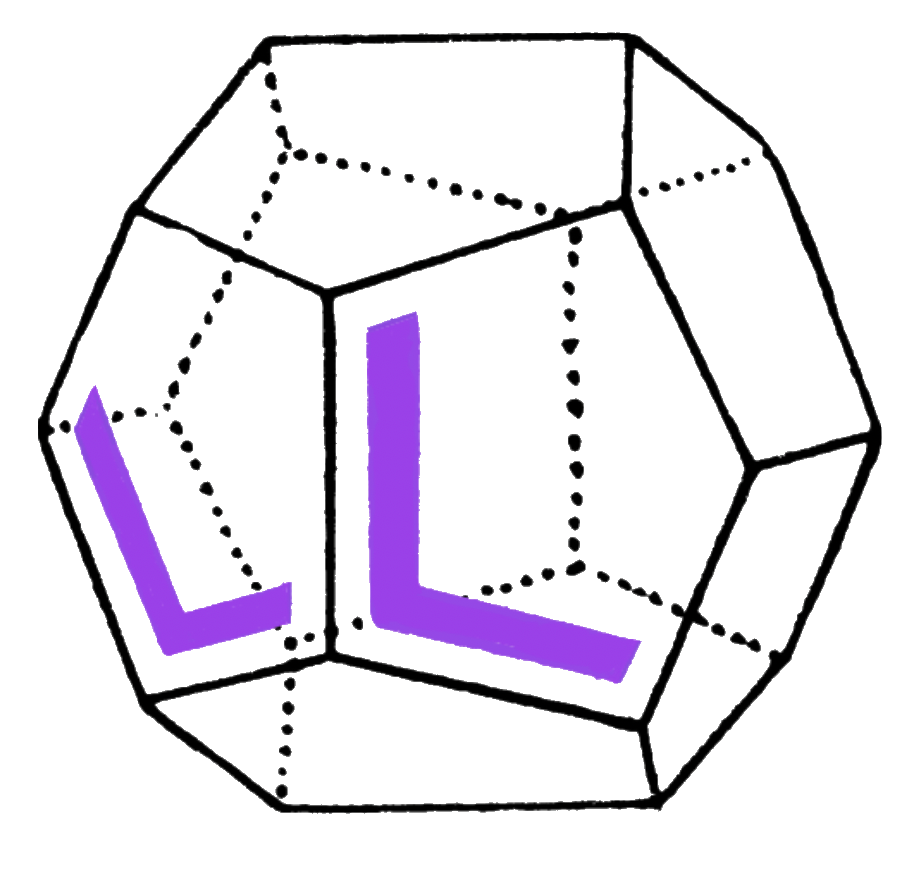
\includegraphics[width=2cm,height=2cm]{ll.png}}

    }}

\AddToShipoutPicture*
  {\put(470,737){

    \href{http://www.linearlibrary.net/CategoryTheory.pdf}{\texttt{.pdf file}}\\

  }}

\AddToShipoutPicture*
  {\put(470,752){
    \href{https://github.com/linlib/CategoryTheory/tree/main}{\texttt{.tex file}}\\

  }}

\AddToShipoutPicture*
  {\put(470,767){
    \href{http://www.linearlibrary.net/CategoryTheory.py}{\texttt{.py file}}

  }}

\AddToShipoutPicture*
  {\put(470,722){
    \href{https://github.com/linlib/CategoryTheory/tree/main}{\texttt{.lean project}}

  }}

\AddToShipoutPicture*
  {\put(470,737){

    \href{http://www.linearlibrary.net/CategoryTheory.pdf}{\texttt{.pdf file}}\\

  }}

\AddToShipoutPicture*
  {\put(415,752){
    \href{https://github.com/linlib/CategoryTheory/tree/main}{\texttt{.java file}}\\

  }}

\AddToShipoutPicture*
  {\put(415,767){
    \href{http://www.linearlibrary.net/CategoryTheory.py}{\texttt{.js file}}

  }}

\AddToShipoutPicture*
  {\put(415,737){
    \href{https://github.com/linlib/CategoryTheory/tree/main}{\texttt{.cpp file}}

  }}

\AddToShipoutPicture*
  {\put(415,722){
    \href{https://github.com/linlib/CategoryTheory/tree/main}{\texttt{.c file}}

  }}

\end{document}







































